\chapter{Supplementary Material for Chapter~\ref{sec:04_models}}
\label{app:04_models}

\section{Message Passing GANs}
\label{app:04_mpgan}

\subsection{Point Cloud Generative Models}
\label{app:04_mpgan_pcgen}

\begin{figure}[htpb!]
    \centering
    \centerline{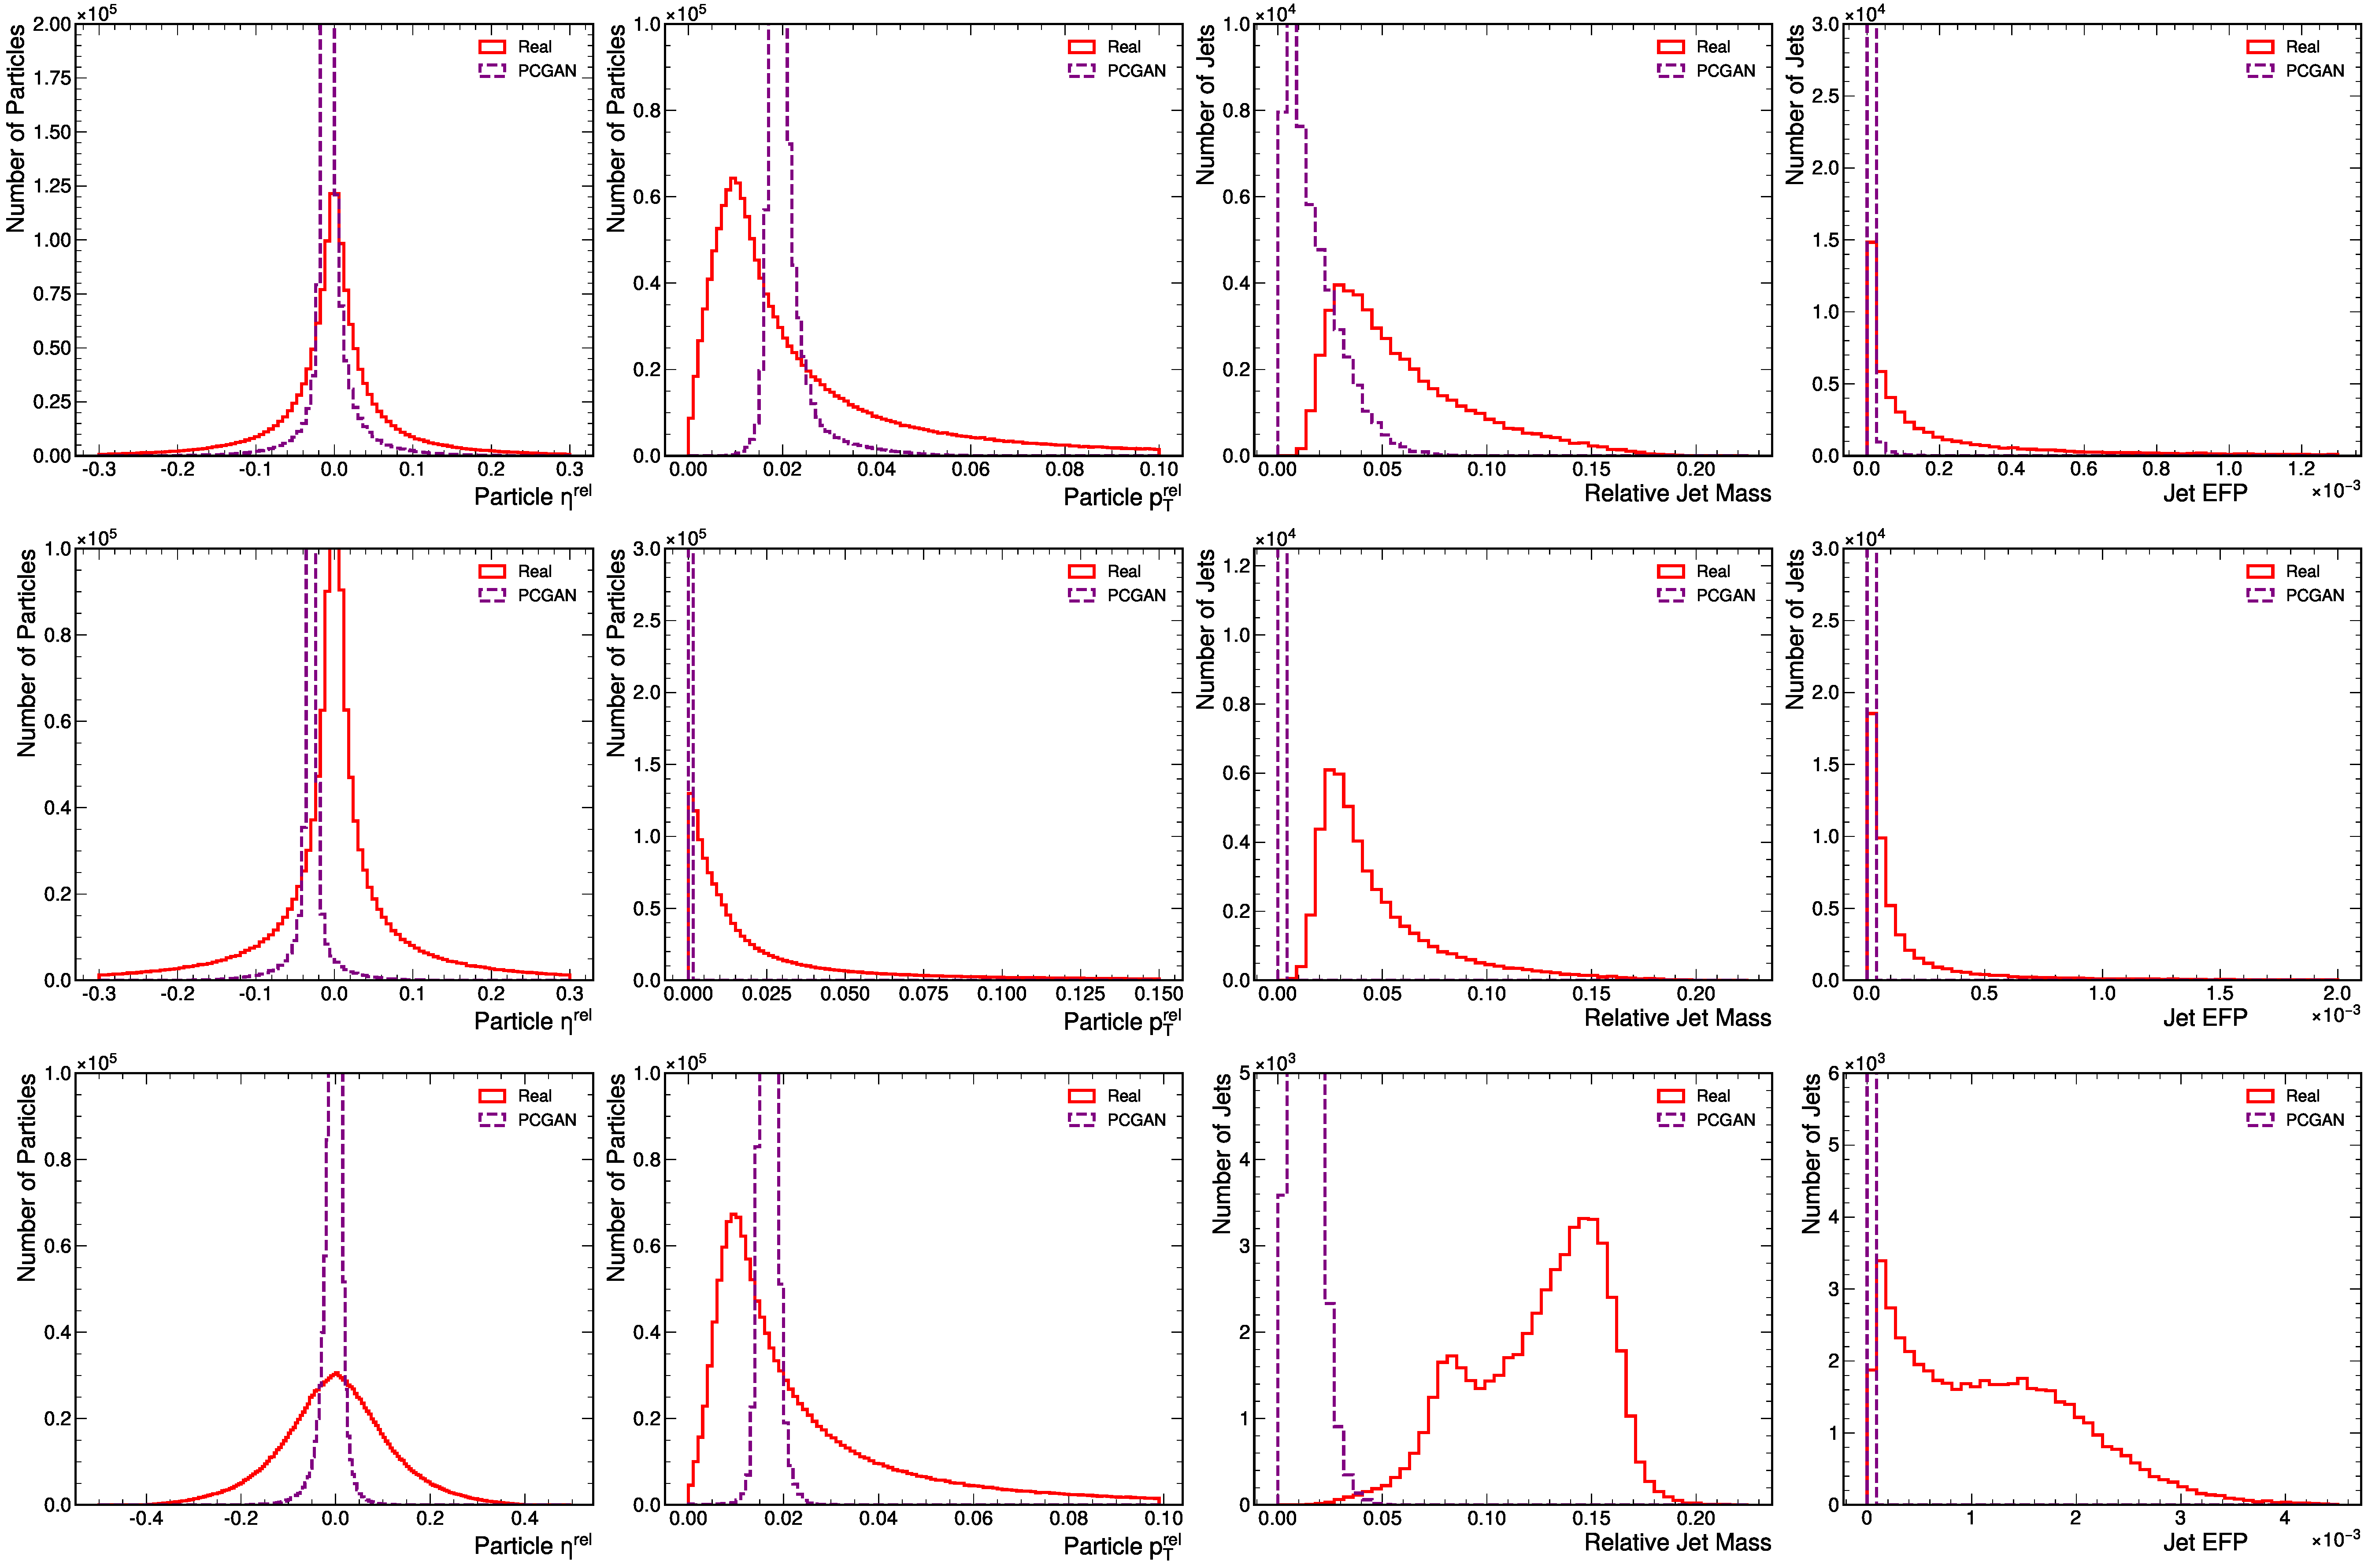
\includegraphics[width=\textwidth]{figures/04-ML4Sim/mpgan/results/pcgan_feature_distributions.pdf}}
    \caption{Comparison of real and PCGAN-generated distributions for a subset of jet and particle features. Top: gluon jet features, Middle: light quark jets, Bottom: top quark jets.}
    \label{fig:04_mpgan_pcgan_results}
\end{figure}

\subsubsection{ShapeNet Point Clouds}
A number of successful generative models exploit a key inductive bias of ShapeNet-based clouds: that the individual distributions of sampled points conditioned on a particular object are identical and independent (the i.i.d assumption). 
This assumption allows for hierarchical generative frameworks, such as Point-Cloud-GAN (PCGAN)~\cite{pcgan}, which uses two networks: one to generate a latent object-level representation, and a second to sample independent points given such a representation.
The PointFlow~\cite{pointflow} and Discrete PointFlow~\cite{discretepointflow} models use a similar idea of sampling independently points conditioned on a learned latent representation of the shape, but with a variational autoencoder (VAE) framework and using normalizing flows for transforming the sampled points. 

This hierarchical-sampling approach is appealing for ShapeNet clouds, however, as discussed in Chapter~\ref{sec:04_mpgan_genhep} the key i.i.d. assumption is not applicable to jets with their highly correlated particle constituents.
In fact, in contrast to ShapeNet objects which have a structure independent of the particular sampled cloud, jets are entirely defined by the distribution of their constituents.

Another model, ShapeGF~\cite{ShapeGF}, uses an approach of again sampling points independently from a prior distribution, but transforming them to areas of high density via gradient ascent, maximizing a learned log-density concentrated on an object's surface.
This approach suffers as well from the i.i.d. assumption in the context of jets, and additionally, unlike for ShapeNet point clouds, there is no such high-density region in momentum-space where particles tend to be concentrated, so learning and maximizing a log-density is not straightforward.

To support our overall claim of the inviability of the i.i.d. assumption for particle clouds, we train a PCGAN model on \jetnet and show the produced feature distributions in Figure~\ref{fig:04_mpgan_pcgan_results}. 
We can see that, as expected, while this network is partially reproducing the particle feature distributions, it is entirely unable to learn the jet-level structure in particle clouds.

\subsubsection{Molecular Point Clouds}

3D molecules are another common point-cloud-style data structure, and there have been developments in generative models in this area as well.
Kohler et al.~\cite{kohler20} introduce physics-motivated normalizing flows equivariant to rotations around the center of mass, i.e. the SO(N) symmetries, for generating point clouds. 
This is appealing as normalizing flows give access to the explicit likelihood of generated samples, and having an architecture equivariant to physical symmetries such as 3D rotations can improve the generalizability and interpretability of the model. 
Since jets are relativistic, however, we require an architecture equivariant to the non-compact SO(3, 1) Lorentz group, to which this model has not been generalized yet. 
Simm et al.~\cite{simm21} present a reinforcement-learning-based approach for generating 3D molecules, using an agent to iteratively add atoms to a molecule and defining the reward function as the energy difference between the new molecule and the old with the new atom at the origin.
This reward function is not directly applicable to jets. where particle distributions are based on the QCD dynamics rather than on minimizing the total energy. 
Finally, Gebauer et al.~\cite{gschnet} introduce G-SchNet, an autoregressive model for producing molecules represented as point clouds, iteratively adding one atom at a time based on the existing molecule. 
Their iterative procedure however was proposed for point clouds of at most nine atoms, and does not scale well in terms of time to larger clouds.

Overall, all the models discussed heavily incorporate inductive biases which are specific to their respective datasets and don't apply to JetNet.
However, they are extremely interesting approaches nonetheless, and adapting them with jet-motivated biases should certainly be explored in future work. 
Indeed, a significant contribution of our work is publishing a dataset which can facilitate and hopes to motivate such development.

\subsection{Training and Implementation Details}
\label{app:04_mpgan_training}

PyTorch code and trained parameters for models in Table~\ref{tab:04_mpgan_results} are provided in the MPGAN repository~\cite{mpgancode}. 
Models were trained and hyperparameters optimized on clusters of NVIDIA GeForce RTX 2080 Ti, Tesla V100, and A100 GPUs. 

\subsubsection{MPGAN}

We use the least squares loss function~\cite{mao_lsgan} and the RMSProp optimizer with a two time-scale update rule~\cite{TTUR} with a learning rate (LR) for the discriminator three times greater than that of the generator. The absolute rate differed per jet type. 
We use LeakyReLU activations (with negative slope coefficient 0.2) after all MLP layers except for the final generator and discriminator outputs where tanh and sigmoid activations respectively are applied. 
We attempted discriminator regularization to alleviate mode collapse via dropout~\cite{srivastava2014dropout}, batch normalization~\cite{ioffe2015batch}, a gradient penalty~\cite{wgangp}, spectral normalization~\cite{spectralnorm}, adaptive competitive gradient descent~\cite{acgd} and data augmentation of real and generated graphs before the discriminator~\cite{karras_2020, tran_2020, zhao_2020}.
Apart from dropout (with fraction $0.5$), none of these demonstrated significant improvement with respect to mode dropping or cloud quality.

We use a generator LR of $10^{-3}$ and train for 2000 epochs for gluon jets, $2\times10^{-3}$ and 2000 epochs for top quark jets, and $0.5\times10^{-3}$ and 2500 epochs for light quark jets. 
We use a batch size of 256 for all jets. 

\subsubsection{rGAN, GraphCNNGAN, TreeGAN, and PointNet-Mix}

For rGAN and GraphCNNGAN we train two variants: (1) using the original architecture hyperparameters in Refs.~\cite{rgan, graphcnngan} for the 2048-node point clouds, and (2) using hyperparameters scaled down to 30-node clouds---specifically: a 32 dimensional latent space, followed by layers of 64, 128, and 90 nodes for r-GAN, or followed by two graph convolutional layers with node features sizes of 32 and 24 respectively for GraphCNN-GAN.
The scaled-down variant performed better for both models, and its scores are the ones reported in Table~\ref{tab:04_mpgan_results}.
For TreeGAN, starting from single vertex---in analogy with a jet originating from a single particle---we use five layers of up-sampling and ancestor-descendant message passing, with a scale-factor of two in each and node features per layer of 96, 64, 64, 64, and 64 respectively.  
LRs, batch sizes, loss functions, gradient penalties, optimizers, ratios of critic to generator updates, activations, and number of epochs are the same as in the original paper and code. 
We use the architecture defined in~\cite{wang2020rethinking} for the PointNet-Mix discriminator. 

\subsubsection{FPND}
\label{app:04_mpgan_pnet}

Apart from the number of input particle features (three in our case, excluding the mask feature), we use the original ParticleNet architecture in Ref.~\cite{Qu:2019gqs}. 
We find training with the Adam optimizer, LR $10^{-4}$, for 30 epochs outperformed the original recommendations on our dataset. 
Activations after the first fully connected layer, pre-ReLU, are used for the FPND measurement.

\subsubsection{PCGAN}
\label{app:04_mpgan_pcgan}

We use the original PCGAN implementation for the sampling networks and training, with a 256-dimensional latent object representation.
For the latent code GAN we use a 3 layer fully connected network for both the generator, with an input size of 128 and intermediate layer sizes of 256 and 512, and discriminator, with intermediate layer sizes of 512 and 256, trained using the Wasserstein-GAN~\cite{WGAN} loss with a gradient penalty.


\subsection{Masking Strategies}
\label{app:04_mpgan_masking}

\begin{figure}[t]
    \centering
    \centerline{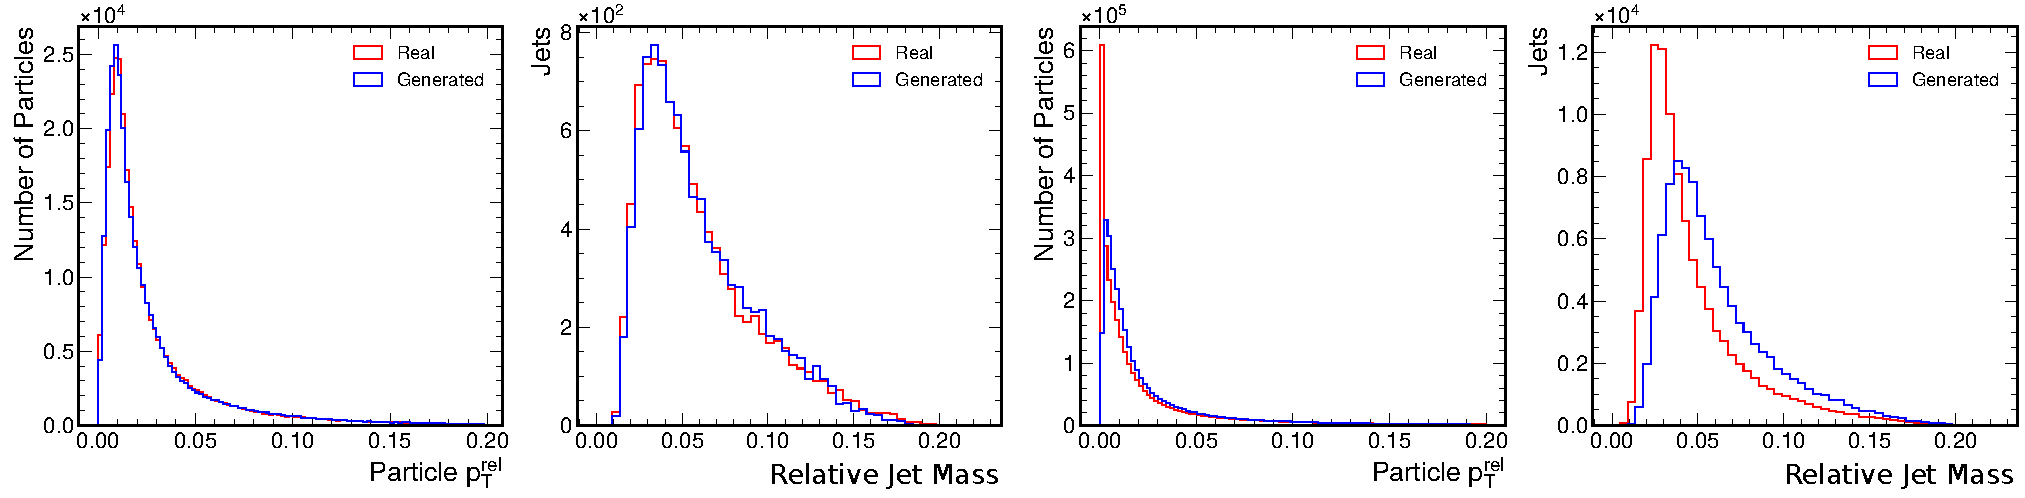
\includegraphics[width=\textwidth]{figures/04-ML4Sim/mpgan/masking/zeropaddingfig.pdf}}
    \caption[Particle $\ptrel$ and relative jet mass distributions of real jets and those generated by MPGAN without our masking strategy.]{Particle $\ptrel$ and relative jet mass distributions of real jets and those generated by MPGAN without our masking strategy. Left: gluon, right: light quark jets.
    We see that while for gluon jets the generator learns distributions correctly, it struggles to learn the discontinuous spike, due to the zero-padded particles, in the light quark $\ptrel$ distribution.
    This also leads to a distorted mass distribution.
    }
    \label{fig:04_mpgan_zeropadding}
\end{figure}

In the \jetnet dataset used for training MPGAN, jets with fewer than 30 particles are zero-padded to fill the 30-particle point cloud. 
Such zero-padded particles pose a problem for the generator, which is not able to learn this sharp discontinuity in the jet constituents (Figure~\ref{fig:04_mpgan_zeropadding}).


\begin{figure}[htpb]
    \centering
    \centerline{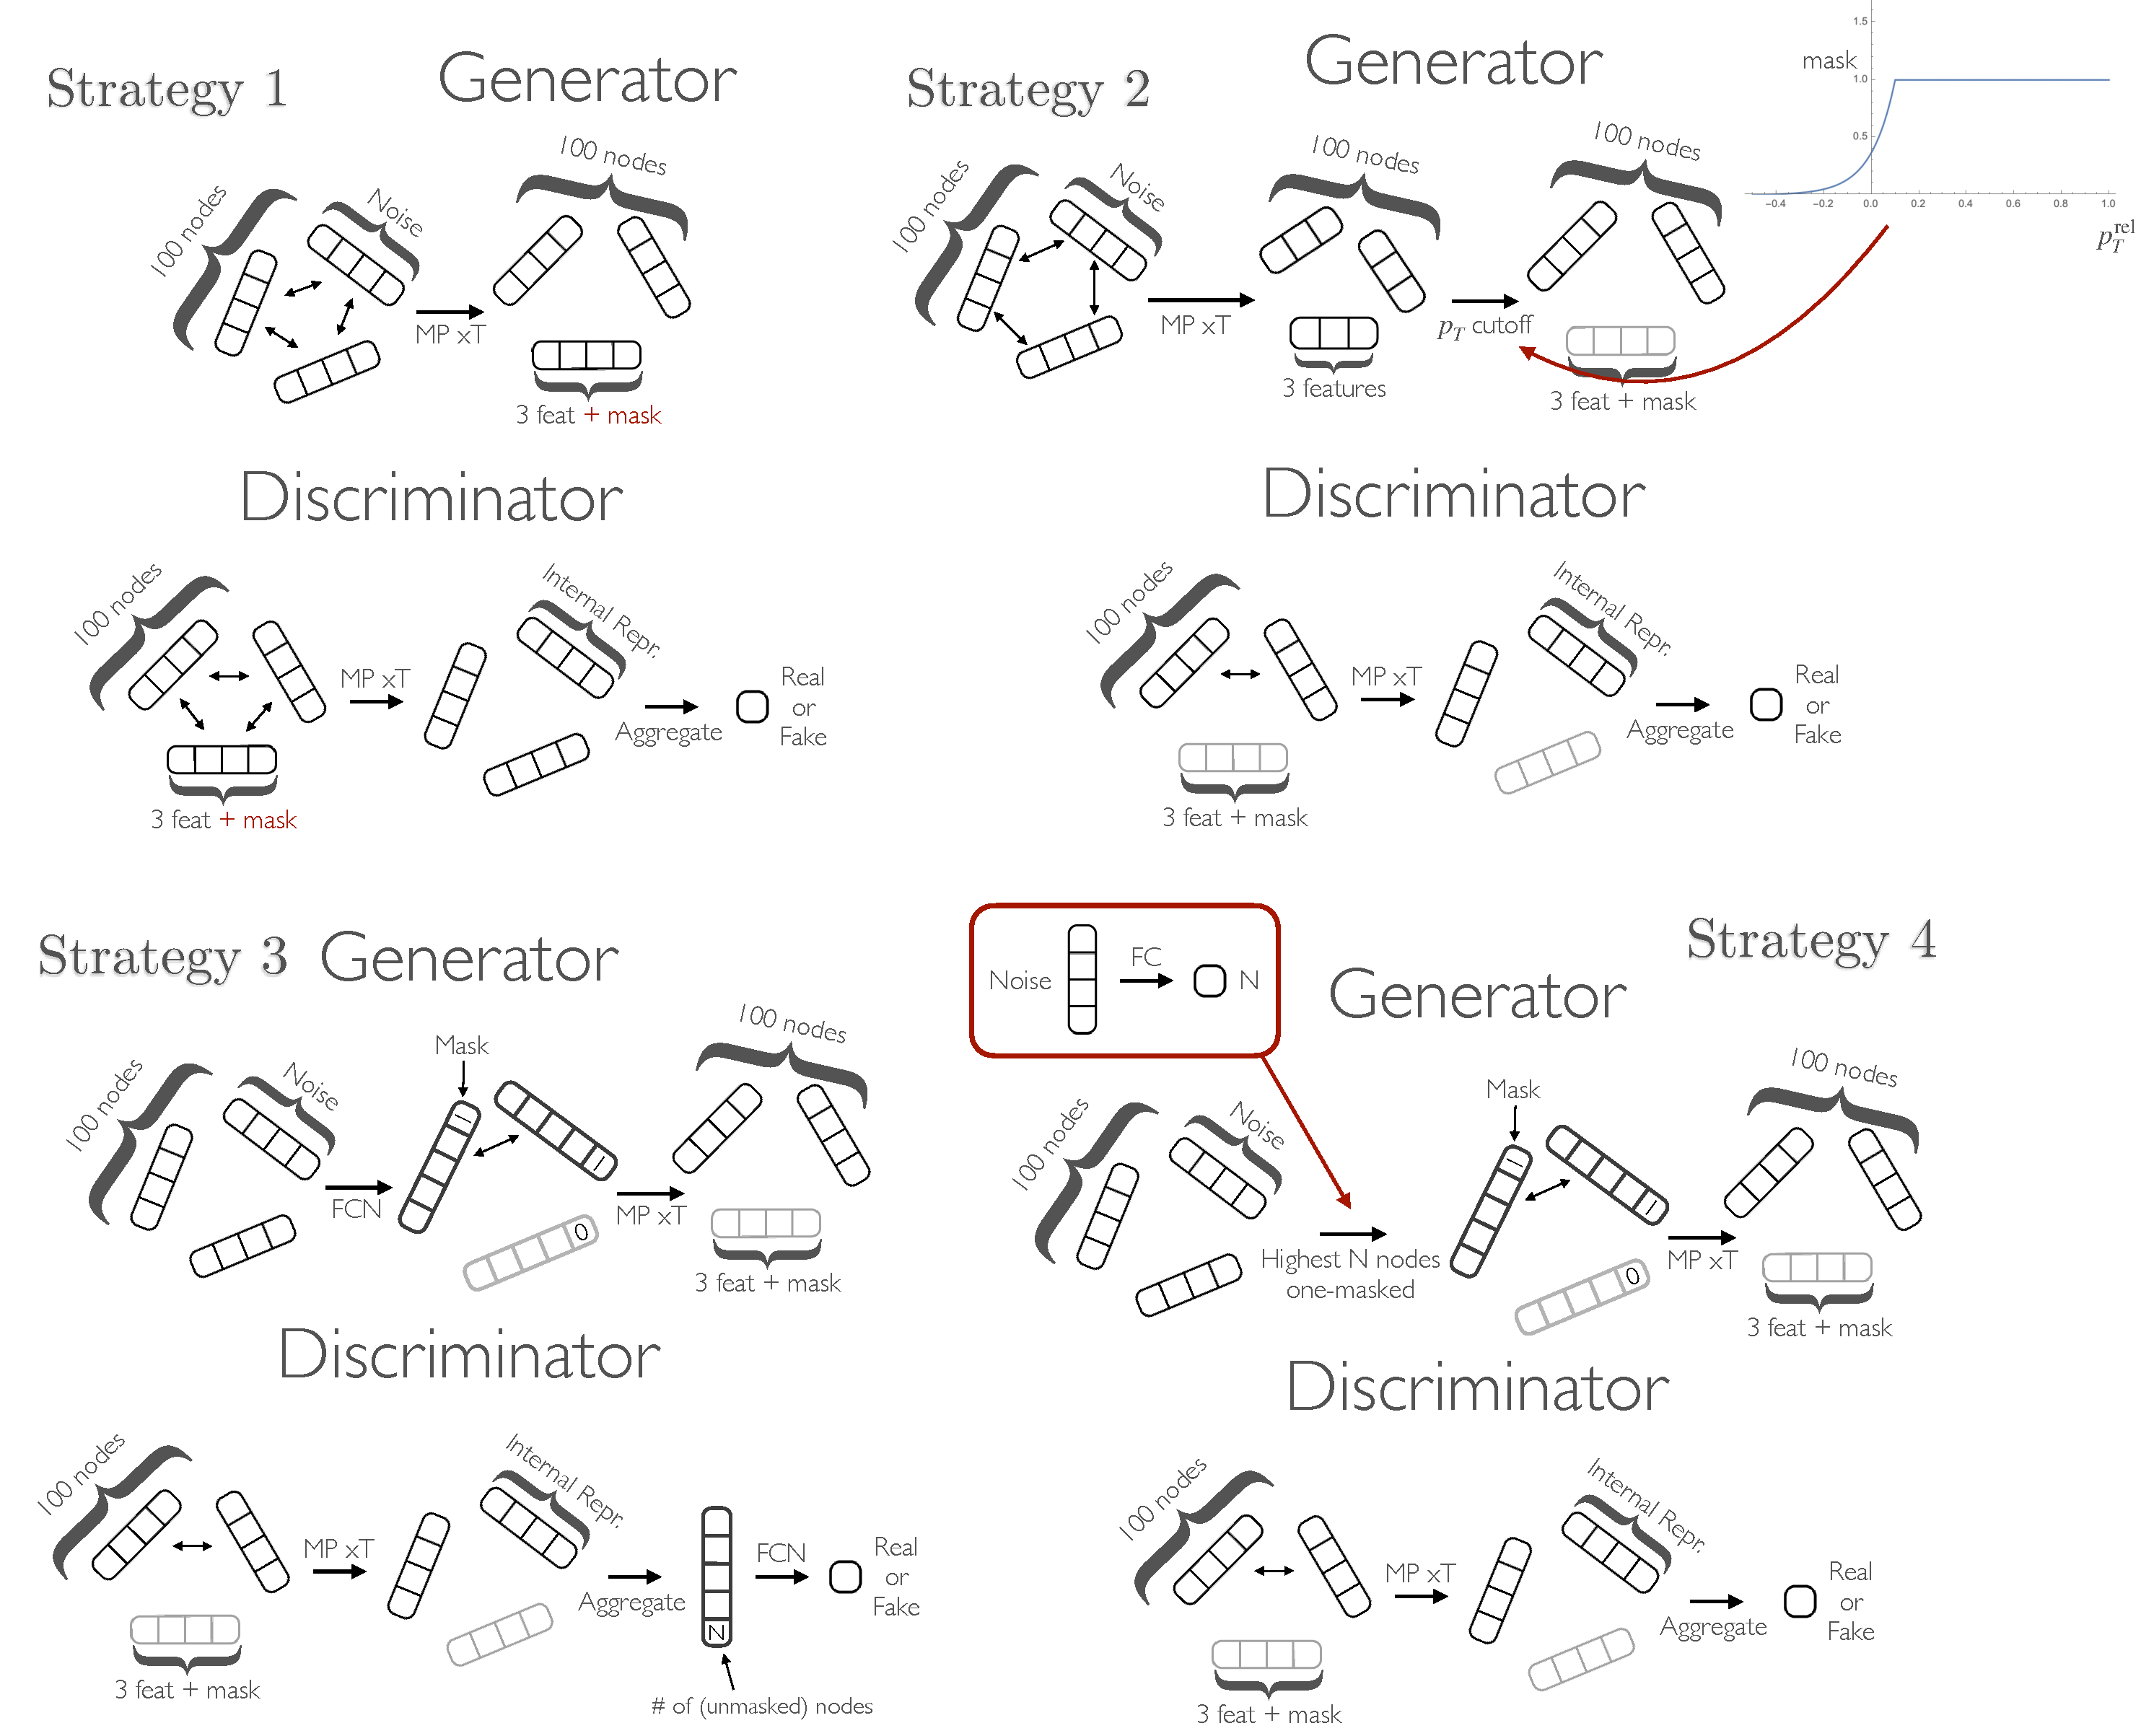
\includegraphics[width=\textwidth]{figures/04-ML4Sim/mpgan/masking/masking.pdf}}
    \caption{The four alternative masking strategies which we test.
    }
    \label{fig:04_mpgan_masking}
\end{figure}

\begin{figure}[htpb]
    \centering
    \centerline{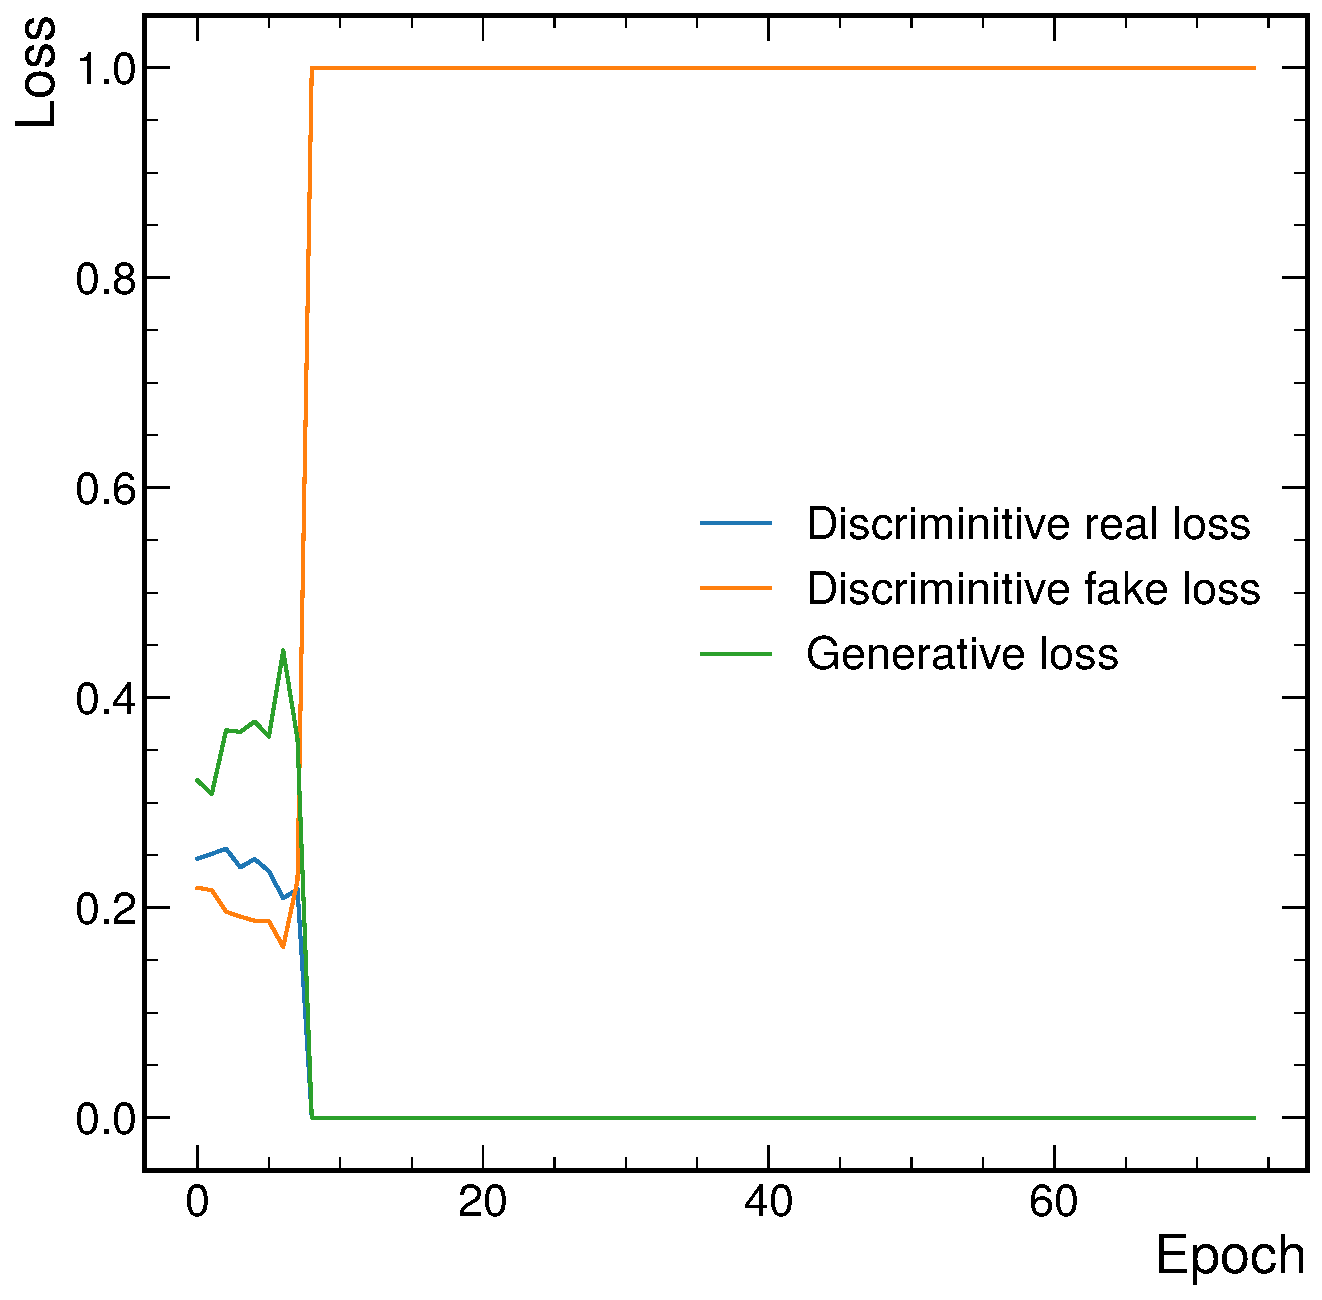
\includegraphics[width=0.6\textwidth]{figures/04-ML4Sim/mpgan/masking/masking_loss.pdf}}
    \caption{Loss curve of a training on light quark jets with masking strategy 3, typical of loss curves with all four strategies.
    }
    \label{fig:04_mpgan_masking_loss}
\end{figure}

To counter this issue, we experiment with five masking strategies, out of which the one described in Section~\ref{sec:04_mpgan_arch} was most successful. 
The four alternatives, which all involve the generator learning the mask without any external input, are shown in Figure~\ref{fig:04_mpgan_masking}.

Strategy 1 treats the mask homogeneously as an extra feature to learn. 
A variation of this weights the nodes in the discriminator the mask. 
In strategy 2, a mask is calculated for each generated particle as a function of its $\ptrel$, based on an empirical minimum cutoff in the dataset. 
In particular, both a Heaviside-step-function and a continuous mask function as in the figure are tested. 
The standard MP discriminator, as described in Section~\ref{sec:04_mpgan_arch}, is used. 
Strategy 3 sees the generator applying an FC layer per particle in the initial cloud to learn their respective masks, with both the MP discriminator, as well as a variant with the number of unmasked nodes in the clouds added as an extra feature to the FC layer. 
In strategies 1 and 3 we test
both binary and continuous masks.
Finally, in strategy 4, we train an auxiliary network to choose a number of particles to mask (as opposed to sampling from the real distribution), which is then passed into the standard MP generator.

We find that all such strategies are unable to produce accurate light quark jets, and in fact trainings for each diverge in the fashion depicted in Figure~\ref{fig:04_mpgan_masking_loss}, even using each discriminator regularization method mentioned in App.~\ref{app:04_mpgan_training}).
We conclude that learning the number of particles to produce is a significant challenge for a generator network, but is a relatively simple feature with which to discriminate between real and fake jets.
To equalize this we use the strategy in Section~\ref{sec:04_mpgan_arch} where the number of particles to produce is sampled directly from the real distribution, removing the burden of learning this distribution from the generator network.

\clearpage
\section{Generative Adversarial Particle Transformers}

\subsection{Results on 150-particle jets}
\label{app:04_gapt_150}

The distributions of real and generated particle and jet features for 150-particle gluon jets by MPGAN and iGAPT are shown in Figure~\ref{fig:04_gapt_feature_distributions_150}.

\begin{figure}[ht]
    \centering
    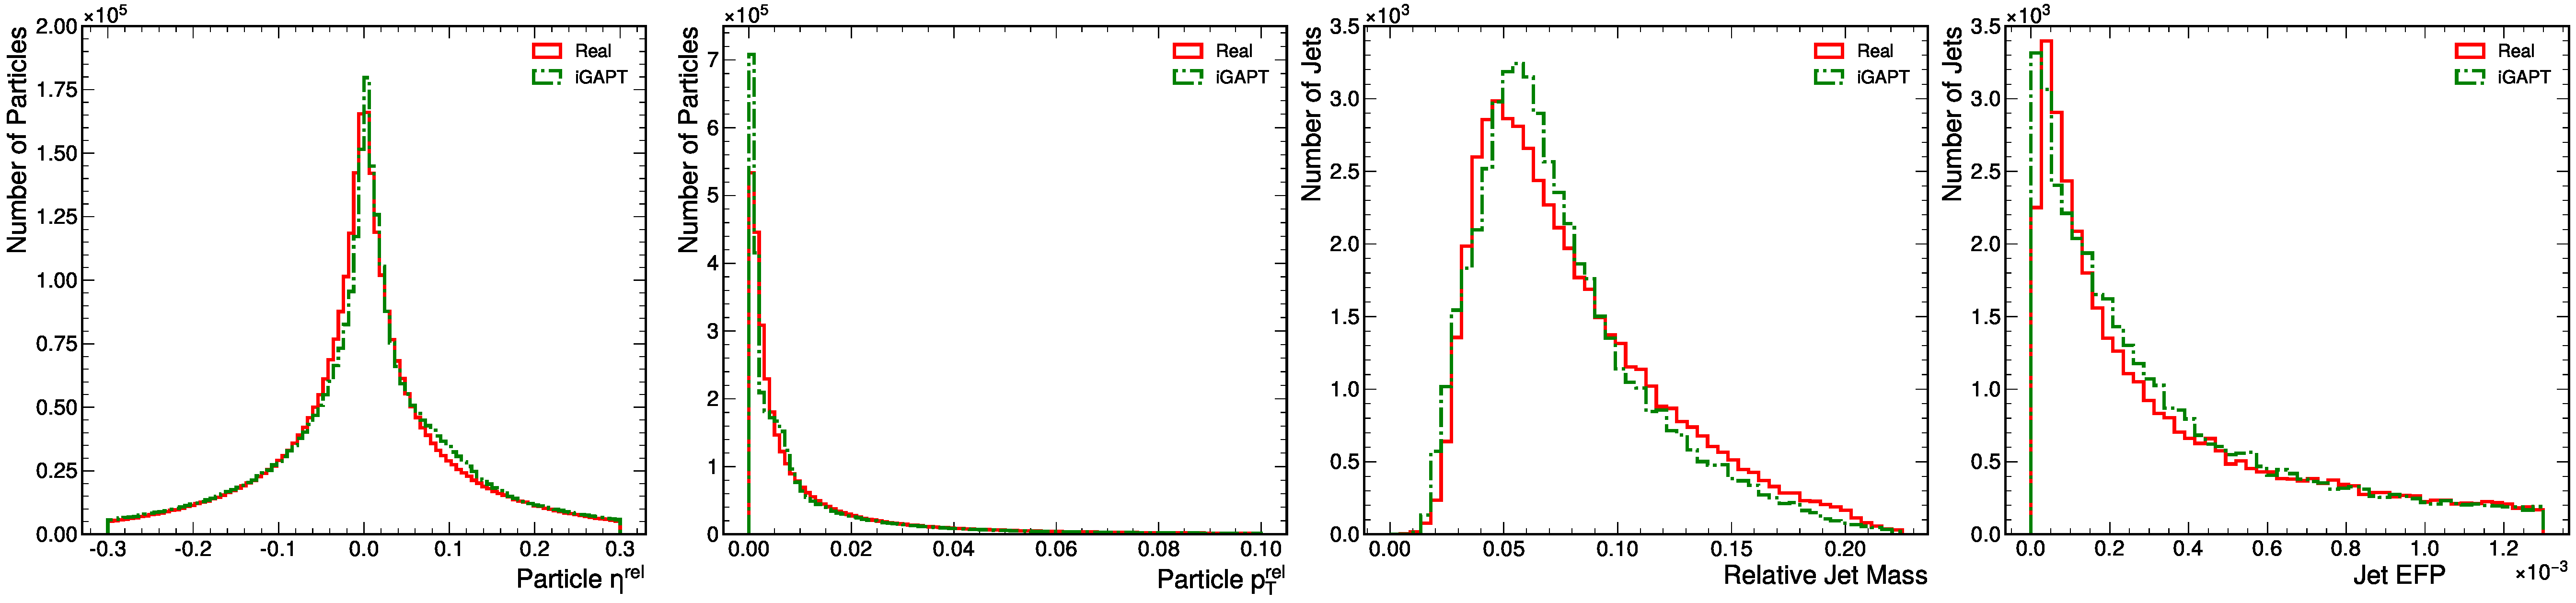
\includegraphics[width=\textwidth]{figures/04-ML4Sim/igapt/feature_distributions_150.pdf}
    \caption[Low-level particle feature distributions and high-level jet feature distributions for 150-particle gluon jets.]{Low-level particle feature distributions (far left and center left) and high-level jet feature distributions (center right and far right) for the real data (red), MPGAN-generated data (blue), and iGAPT-generated data (green), for 150-particle gluon jets.
    A sample $d = 4$ energy flow polynomial~\cite{Komiske:2017aww} is chosen in the rightmost column.
    }
    \label{fig:04_gapt_feature_distributions_150}
\end{figure}


\chapter{Supplementary Material for Chapter~\ref{sec:04_evaluating}}

\section{Further Discussion on IPMs vs. \texorpdfstring{$f$}{f}-Divergences}
\label{app:04_evaluating_metricspace} 

A crucial advantage of IPMs in evaluating generative models is that they consider the metric space of the distributions.
We illustrate this with the help of Figure~\ref{fig:04_evaluating_metricspace}, inspired heavily by Refs.~\cite{gretton_talk, w1_stackoverflow}, which shows an example real (in red) and two generated (in blue) jet mass distributions.
Clearly, in the context of simulation, the second generated distribution contains a peak closer to the real peak and, hence, is a better model.
However, because $f$-divergences such as the KL or $\chi^2$ look only at the pointwise difference between distributions, they find both generated distributions to be as discrepant with the real.
IPMs like the Wasserstein metric or MMD, on the other hand, generally identify the second distribution as being closer to the real.

\begin{figure*}[htpb]
    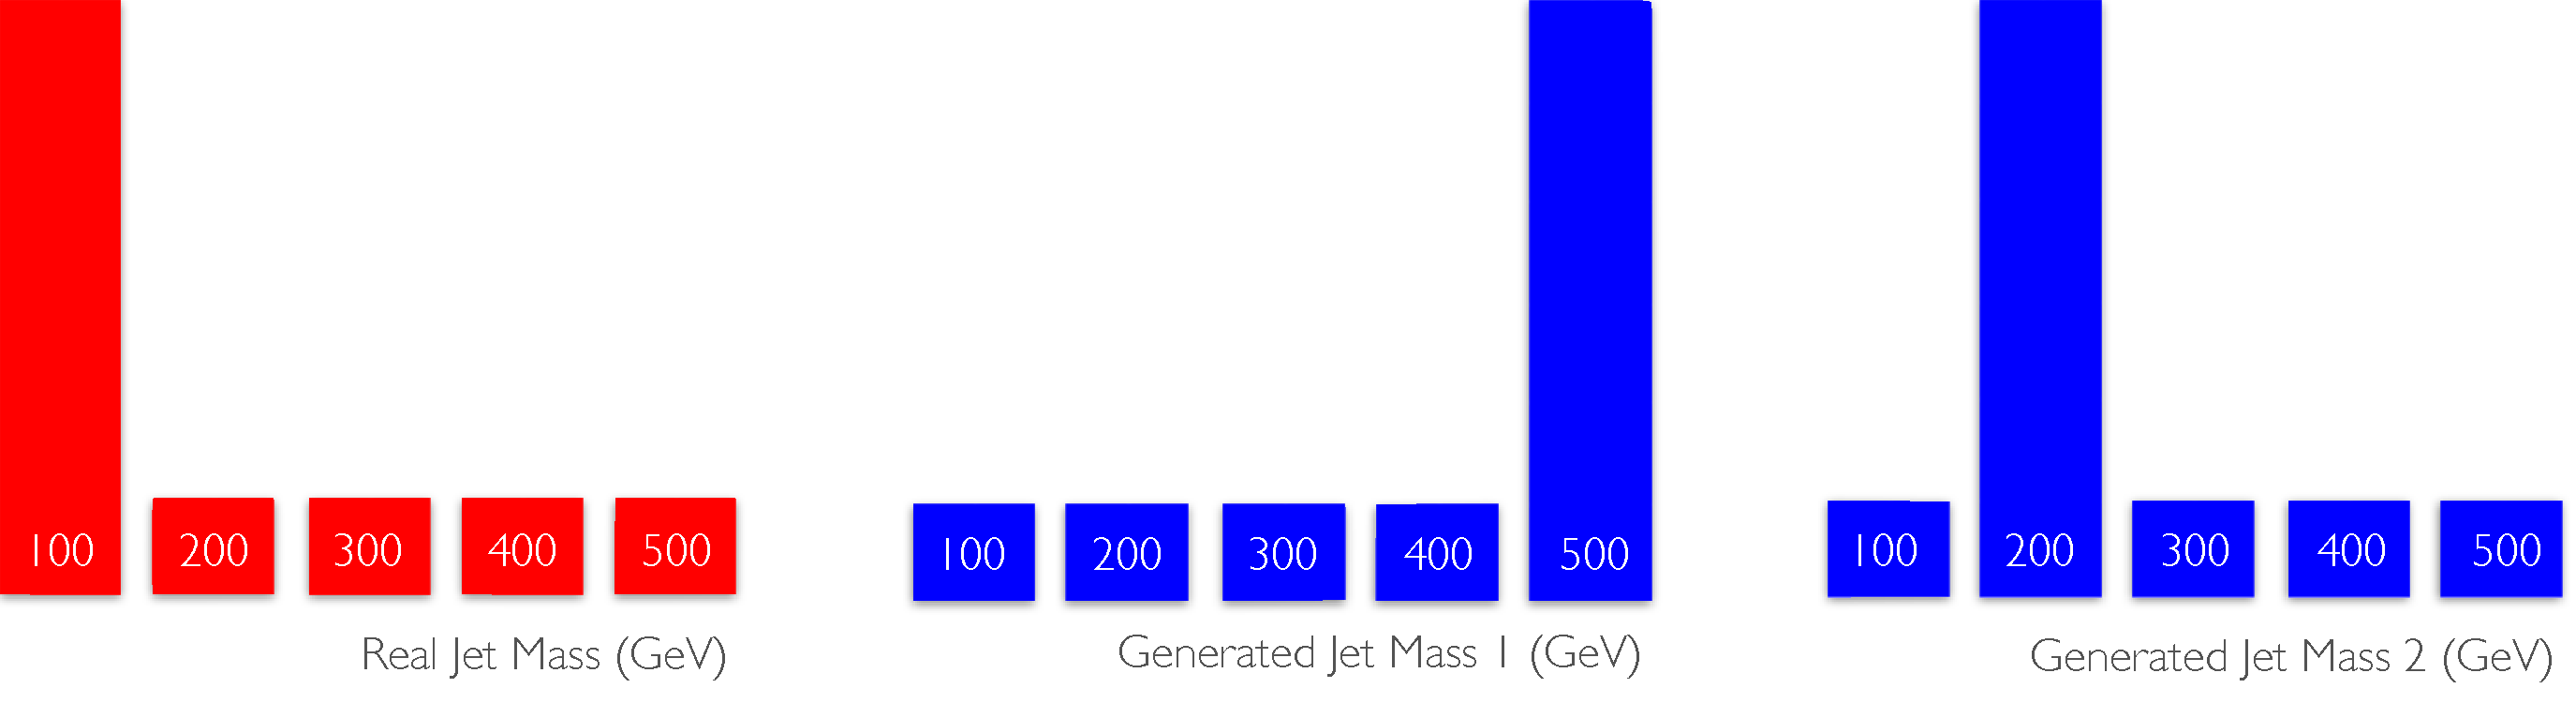
\includegraphics[width=\textwidth]{figures/04-ML4Sim/evaluating/metricspace.pdf}
    \caption{Example real and generated jet mass distributions used to illustrate the benefit of IPMs in Appendix~\ref{app:04_evaluating_metricspace}, based on Refs.~\cite{gretton_talk, w1_stackoverflow}.}
    \label{fig:04_evaluating_metricspace}
\end{figure*}

\section{Further Discussion on Gaussian Dataset Experiments}
\label{app:04_evaluating_details} 

\begin{figure*}[htpb]
    \centering
    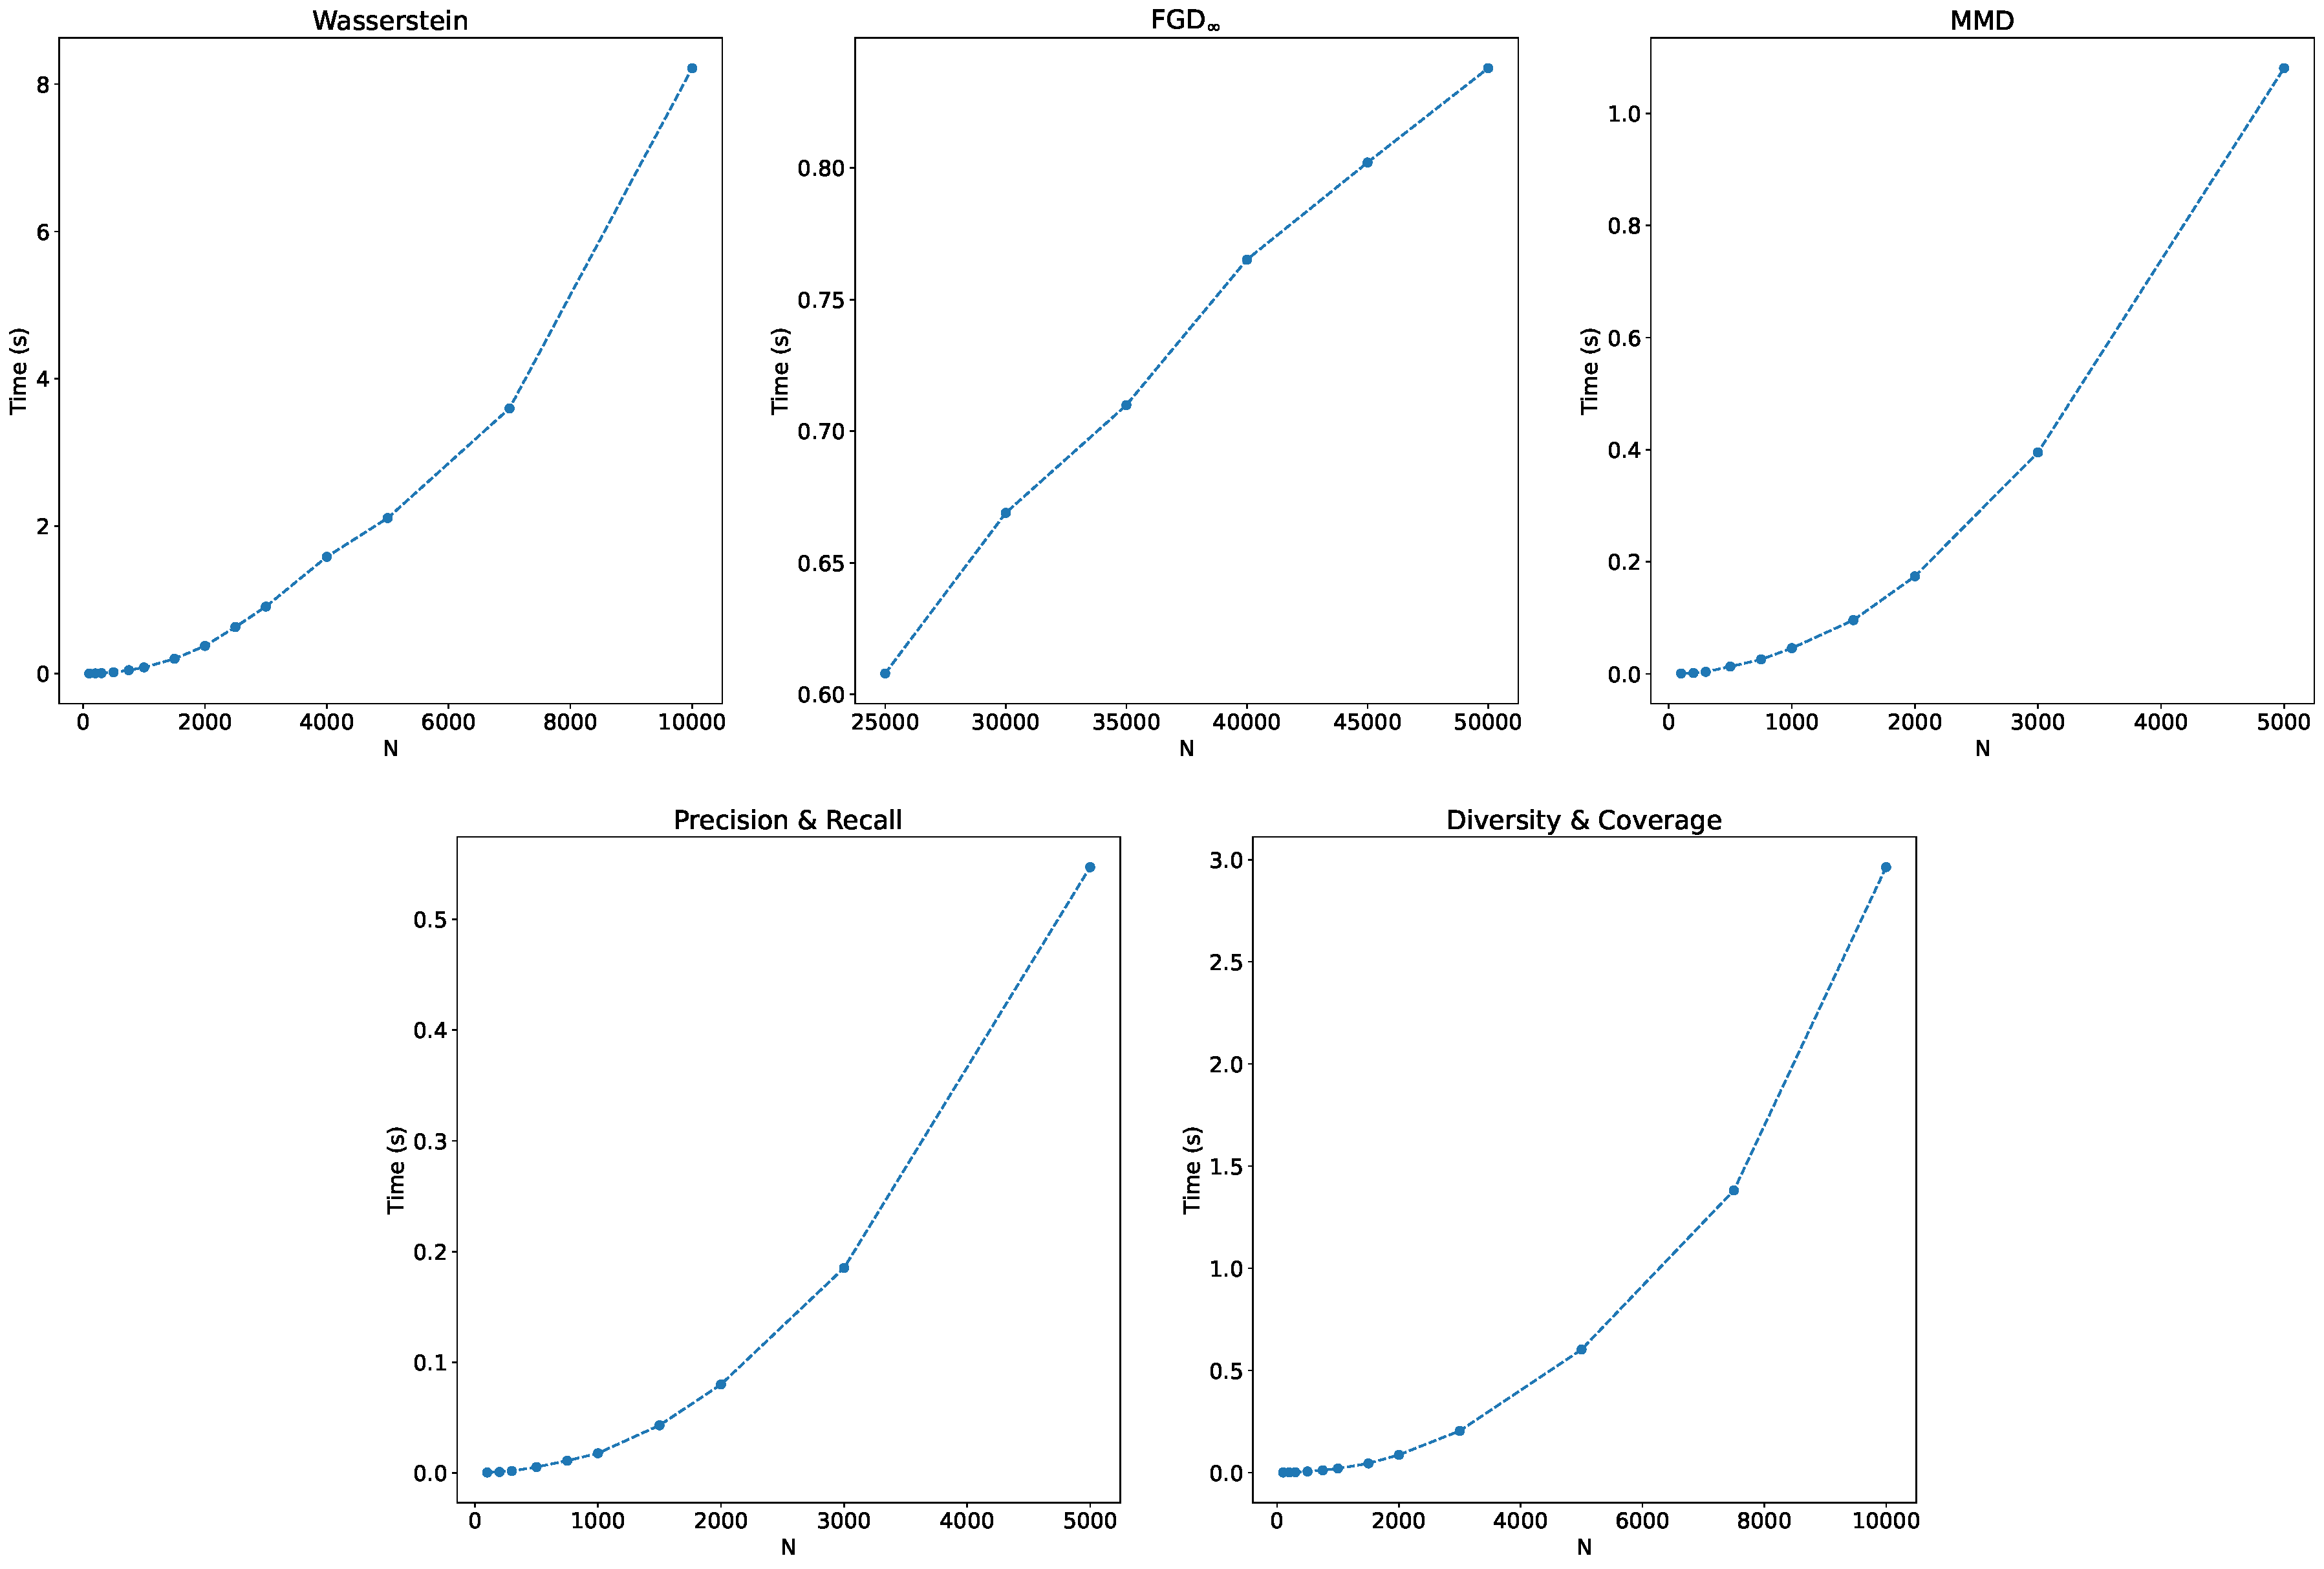
\includegraphics[width=\textwidth]{figures/04-ML4Sim/evaluating/timings.pdf}
    \caption{Time taken per each metric on Gaussian-distributed datasets as described in Section~\ref{sec:04_evaluating_toydata}.}
    \label{fig:04_evaluating_timings}
\end{figure*}

\begin{figure*}[htpb]
    \centering
    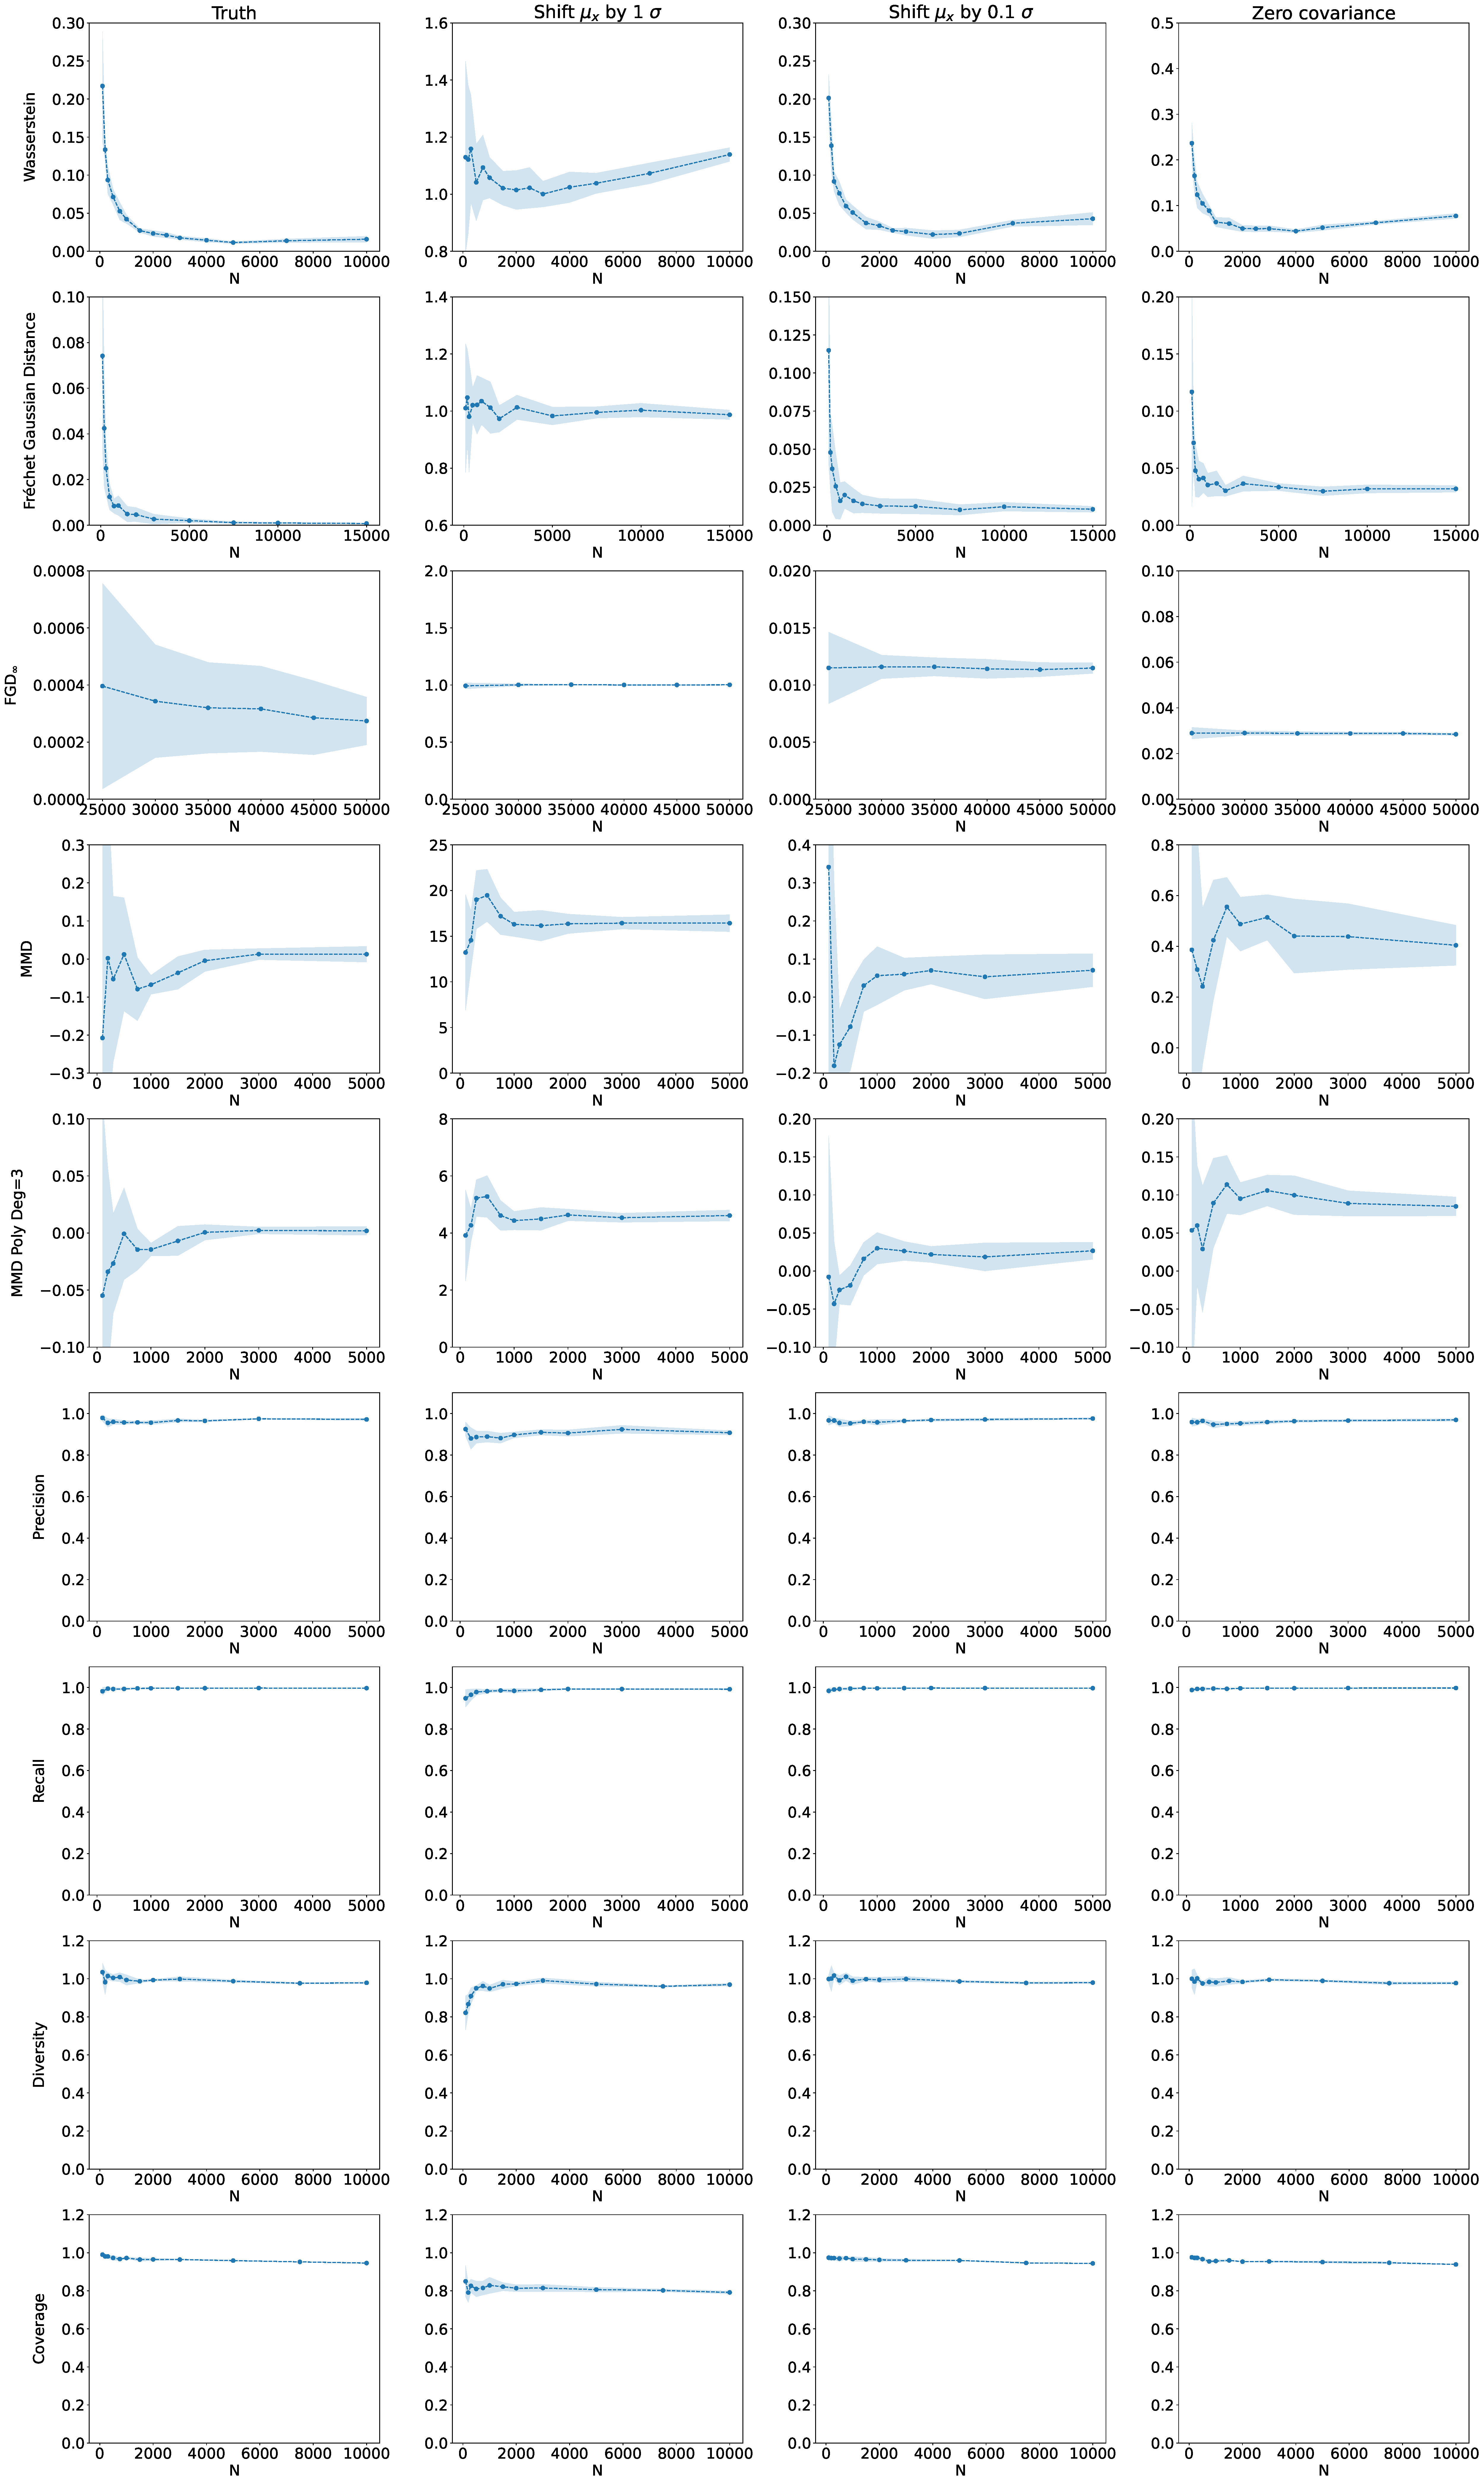
\includegraphics[width=0.75\textwidth]{figures/04-ML4Sim/evaluating/toy_scores_1.pdf}
    \caption{Scores of each metric on Gaussian-distributed datasets as described in Section~\ref{sec:04_evaluating_toydata}.}
    \label{fig:04_evaluating_toyscores1}
\end{figure*}

\begin{figure*}[htpb]
    \centering
    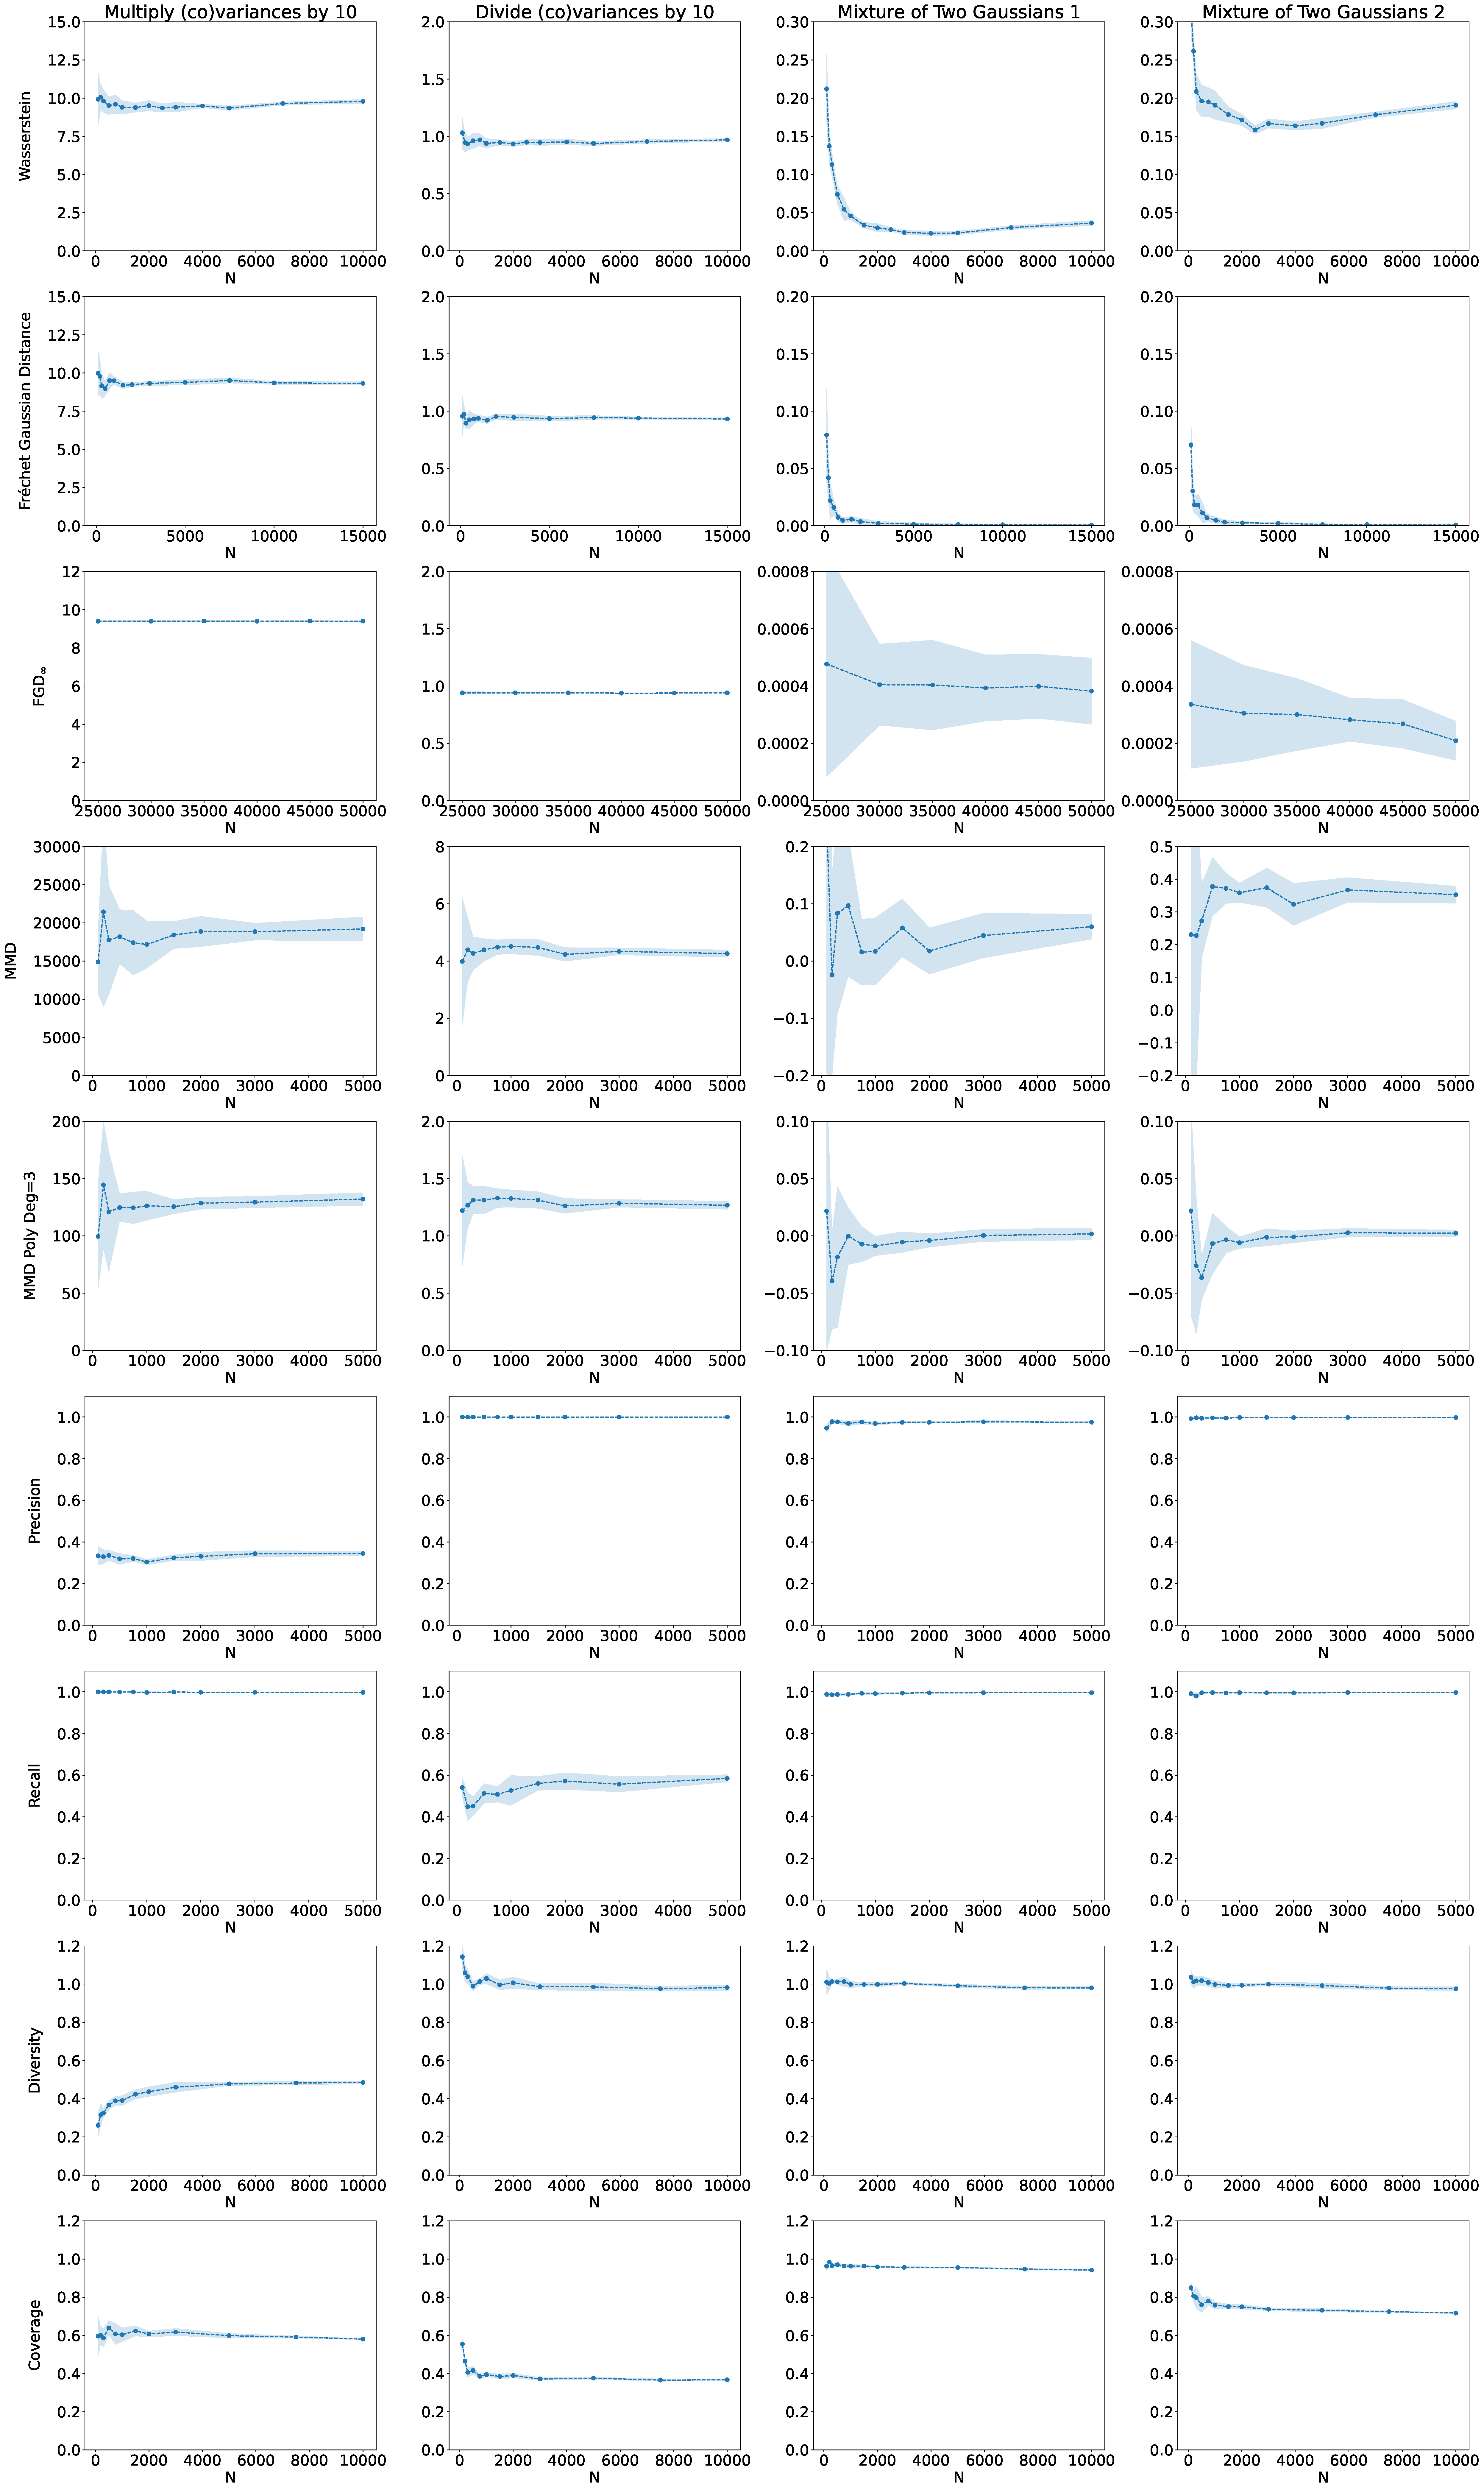
\includegraphics[width=0.75\textwidth]{figures/04-ML4Sim/evaluating/toy_scores_2.pdf}
    \caption{Scores of each metric on Gaussian-distributed datasets as described in Section~\ref{sec:04_evaluating_toydata}.}
    \label{fig:04_evaluating_toyscores2}
\end{figure*}

Figure~\ref{fig:04_evaluating_timings} plots the time taken per measurement of each metric used in Section~\ref{sec:04_evaluating_toydata} for different sample sizes, measured on an 8-core Intel Core i9 processor.
The quadratic scaling of the Wasserstein and diversity and coverage metrics, in combination with their low rate of convergence, means their use for evaluation is practically difficult.
MMD and precision and recall exhibit the same scaling; however, are observed to converge within roughly 3000 samples.
\fgdinf scales linearly and remains fast to compute even at the highest batch size tested.

Figures~\ref{fig:04_evaluating_toyscores1} and~\ref{fig:04_evaluating_toyscores2} show measurements of each metric on each distribution discussed in Section~\ref{sec:04_evaluating_toydata}, as well as FGD and MMD with a third-order polynomial kernel for varying samples sizes.
We can see from these plots that indeed, as discussed in Refs.~\cite{binkowski_demystifying, chong_unbiasedfid}, FGD is biased, but the solution from Ref.~\cite{chong_unbiasedfid} of extrapolating to infinite-sample size (\fgdinf) largely solves this issue.
We also note that, perhaps surprisingly, a third-order polynomial kernel, as used for the KID~\cite{binkowski_demystifying} in computer vision, is not sufficient to discern the mixtures of Gaussian distributions from the single Gaussian.
Hence, we recommend a fourth-order kernel for the kernel physics distance.

\section{Alternative Jet Distributions}
\label{app:04_evaluating_jet_plots} 


Distributions of particle- and jet-level features from the true and distorted jets as described in Section~\ref{sec:04_evaluating_jetdata} are shown in Figure~\ref{fig:04_evaluating_jet_dists_app}.\\

\begin{figure*}[htpb]
    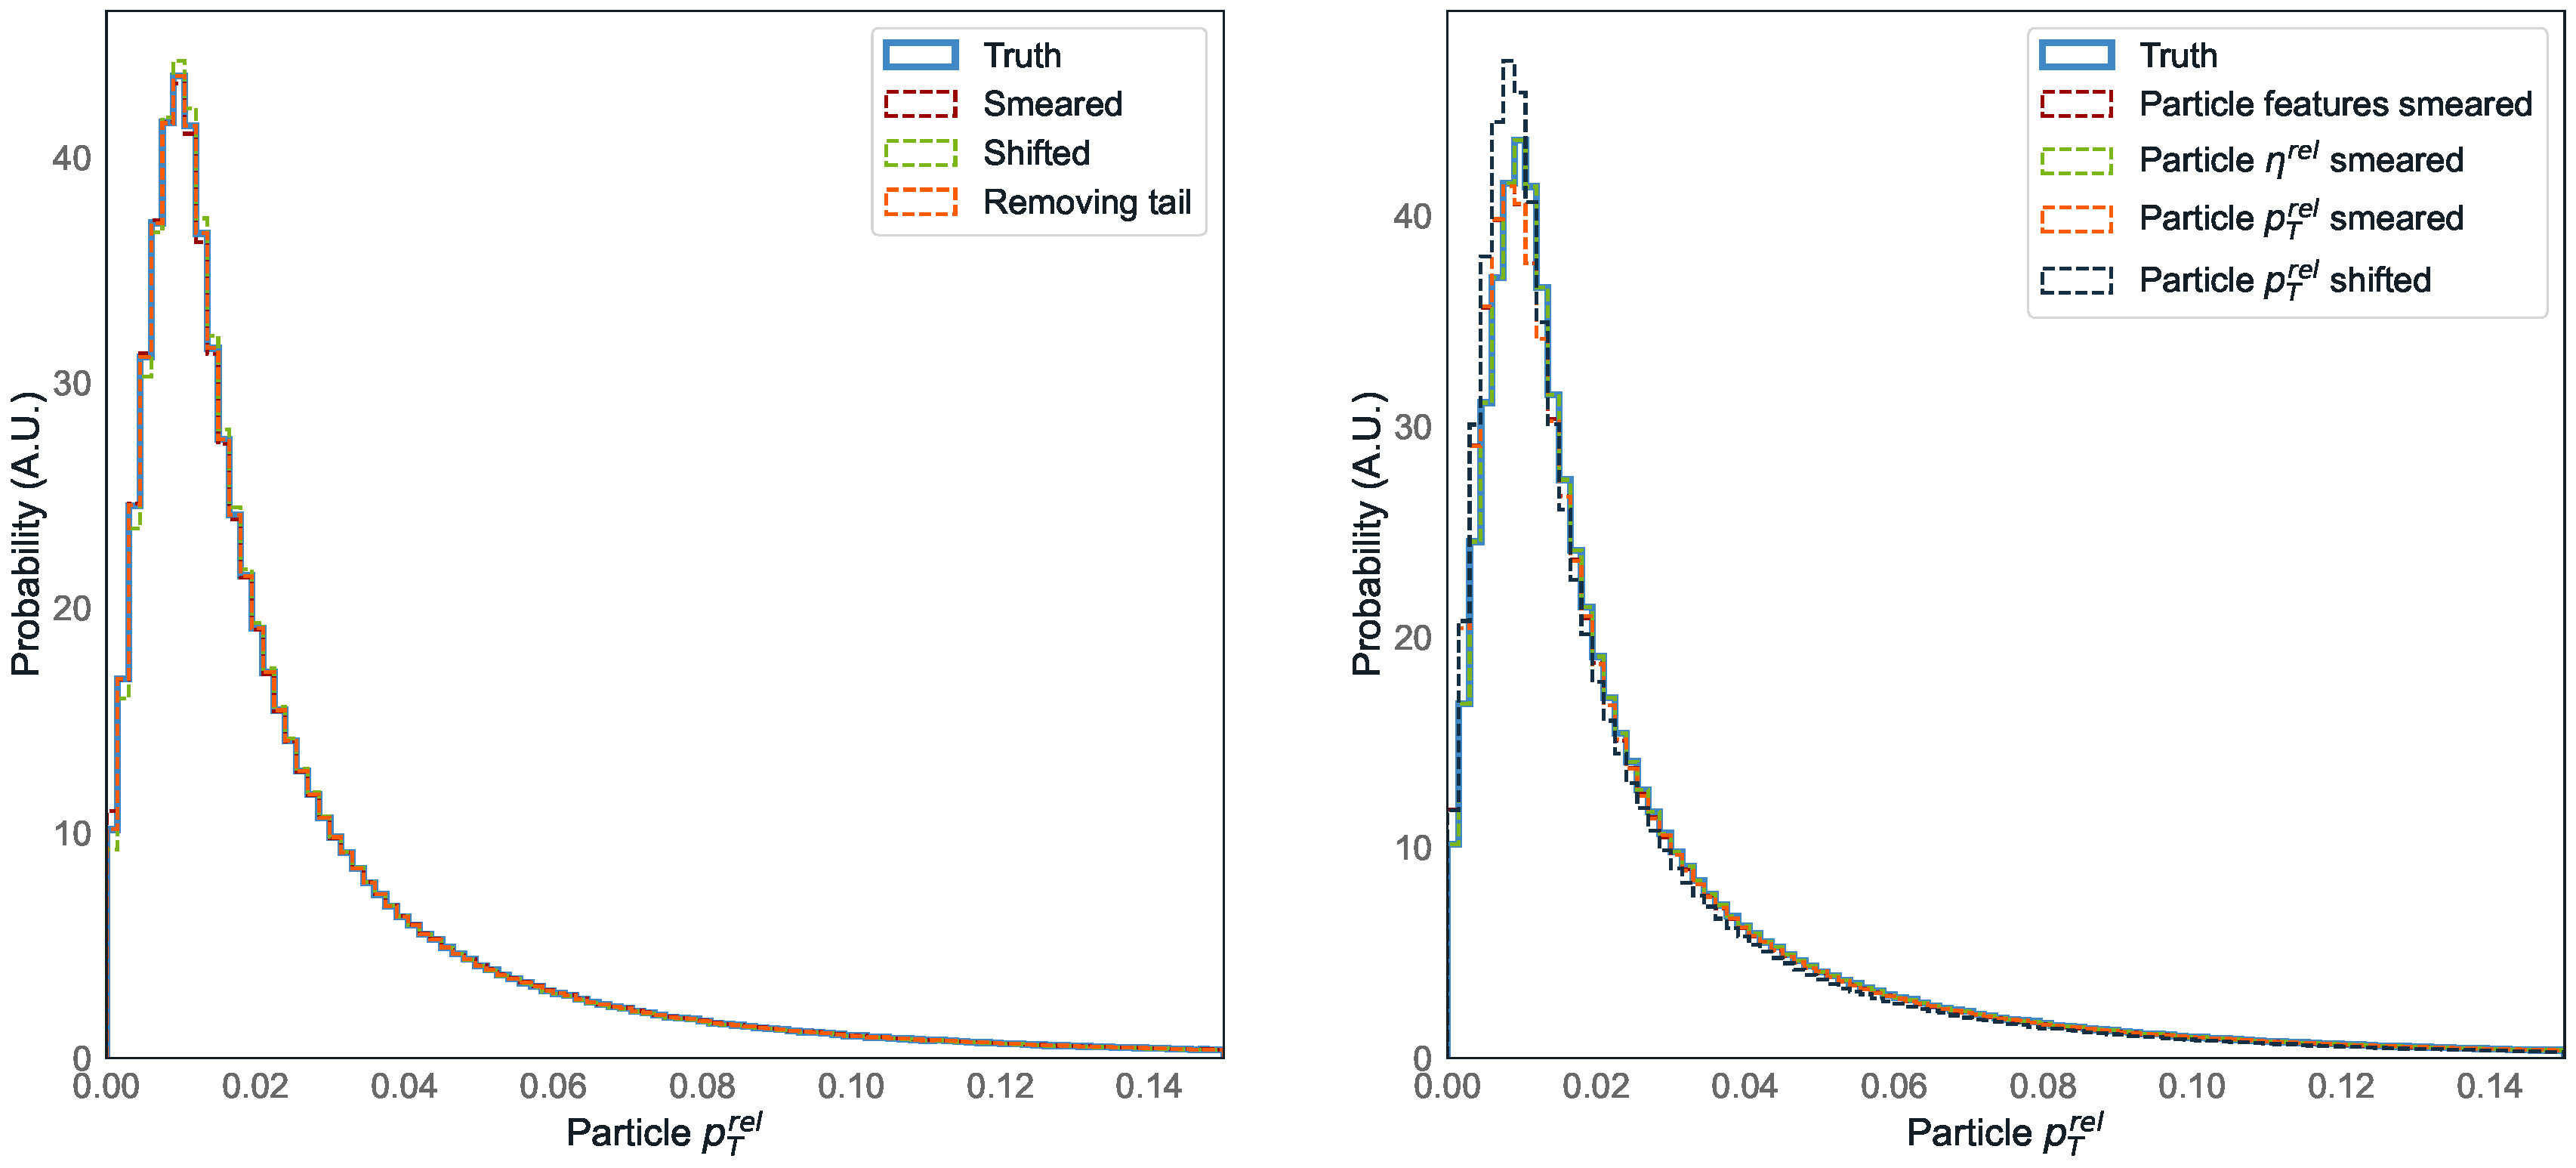
\includegraphics[width=0.94\textwidth]{figures/04-ML4Sim/evaluating/jet_partpt_dists.pdf}
    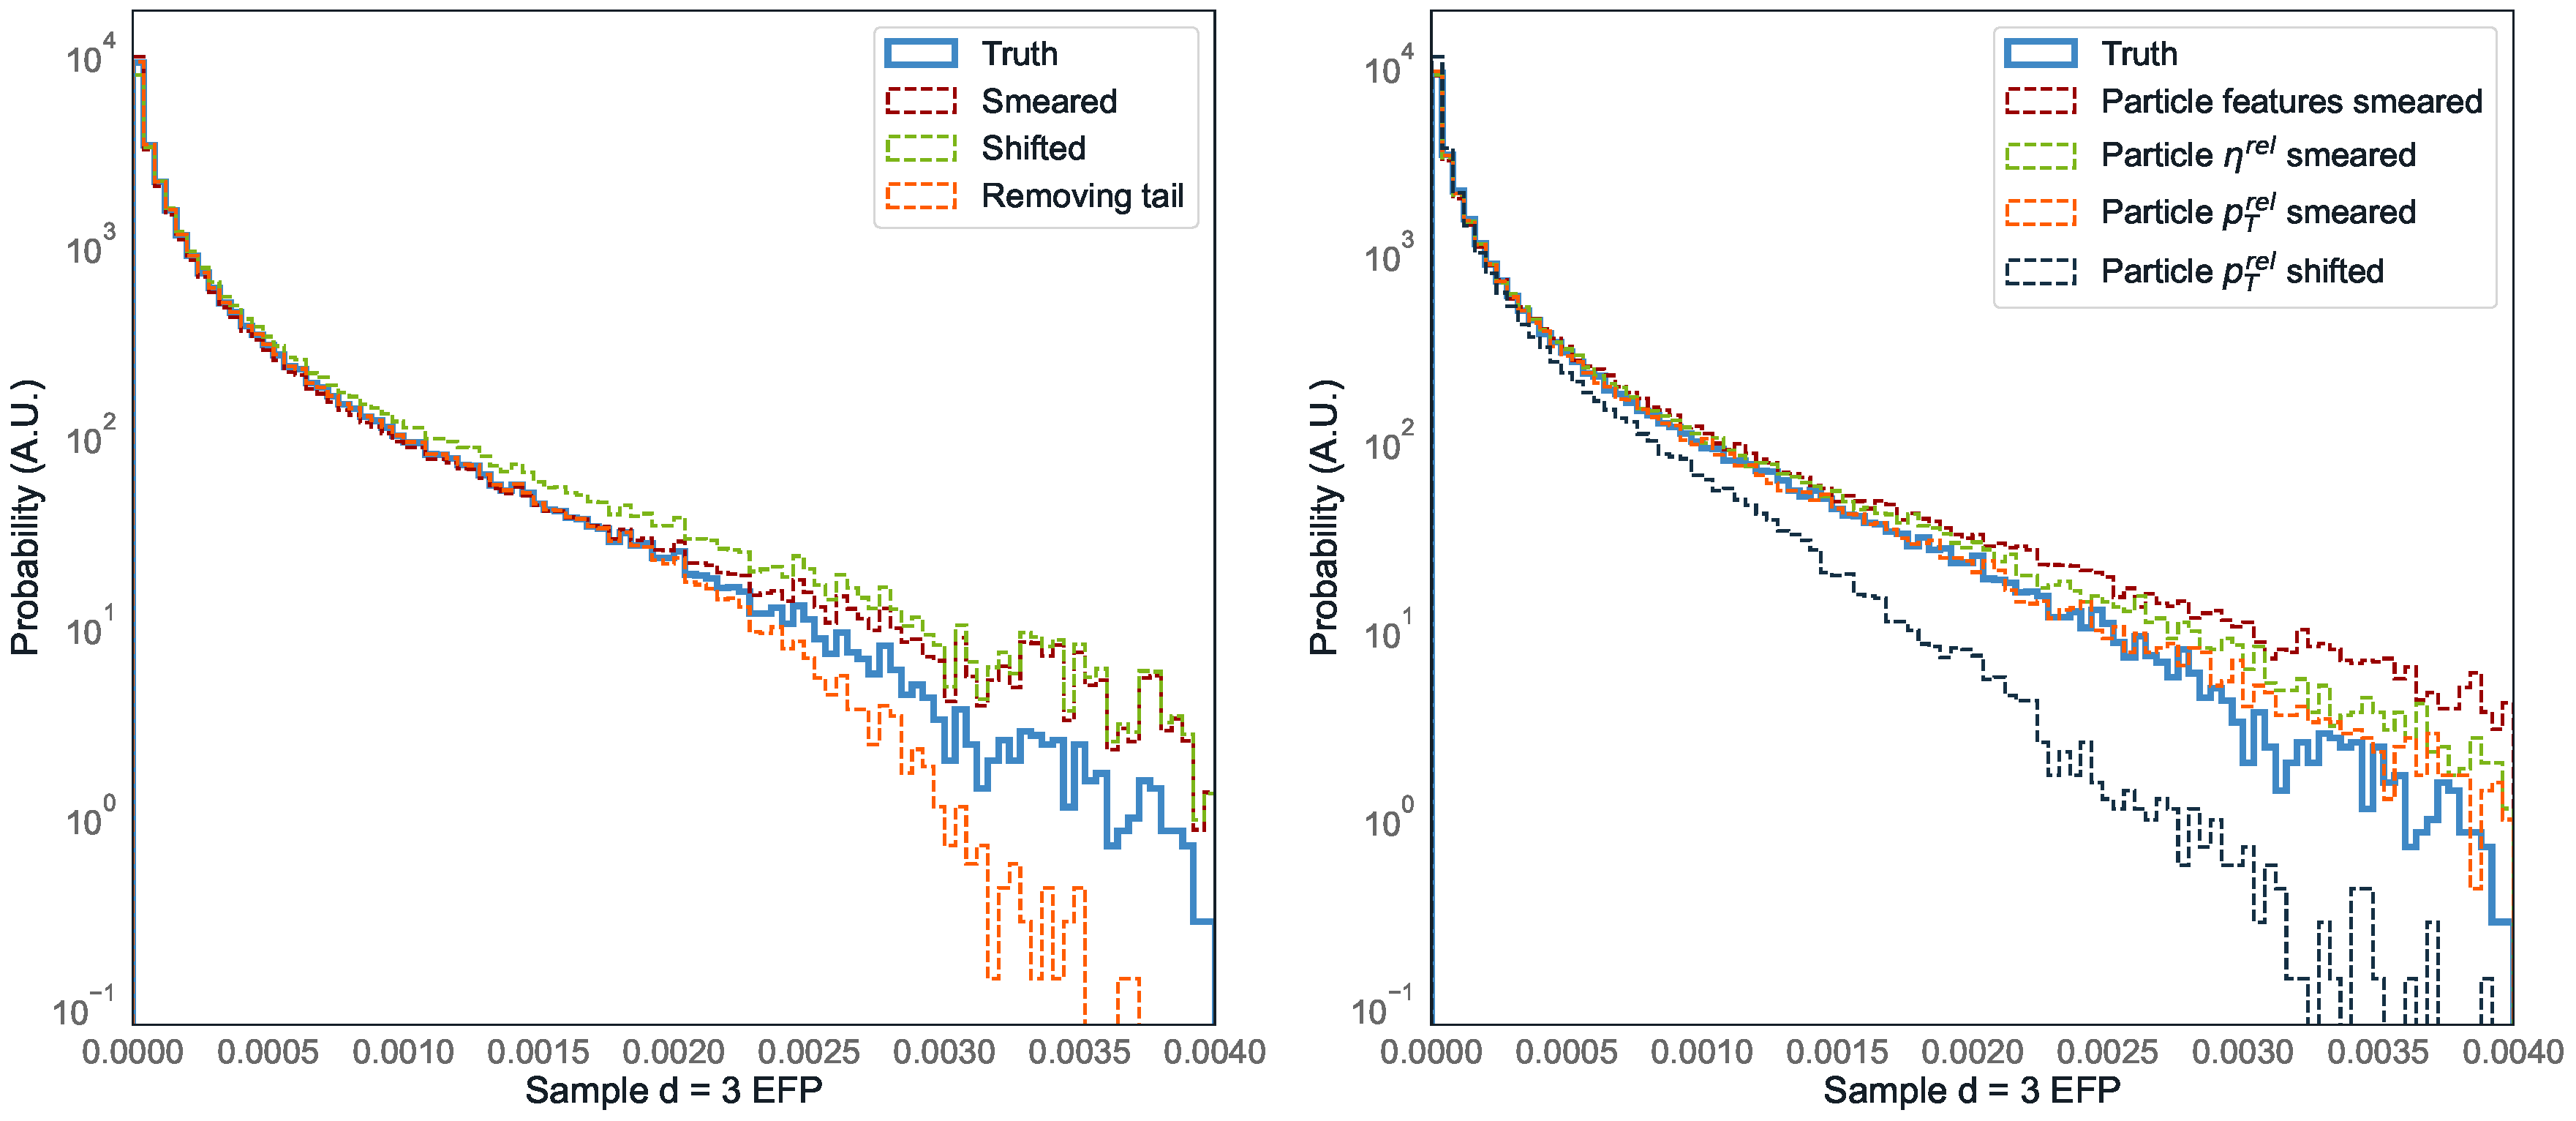
\includegraphics[width=0.94\textwidth]{figures/04-ML4Sim/evaluating/jet_efp12_dists.pdf}
    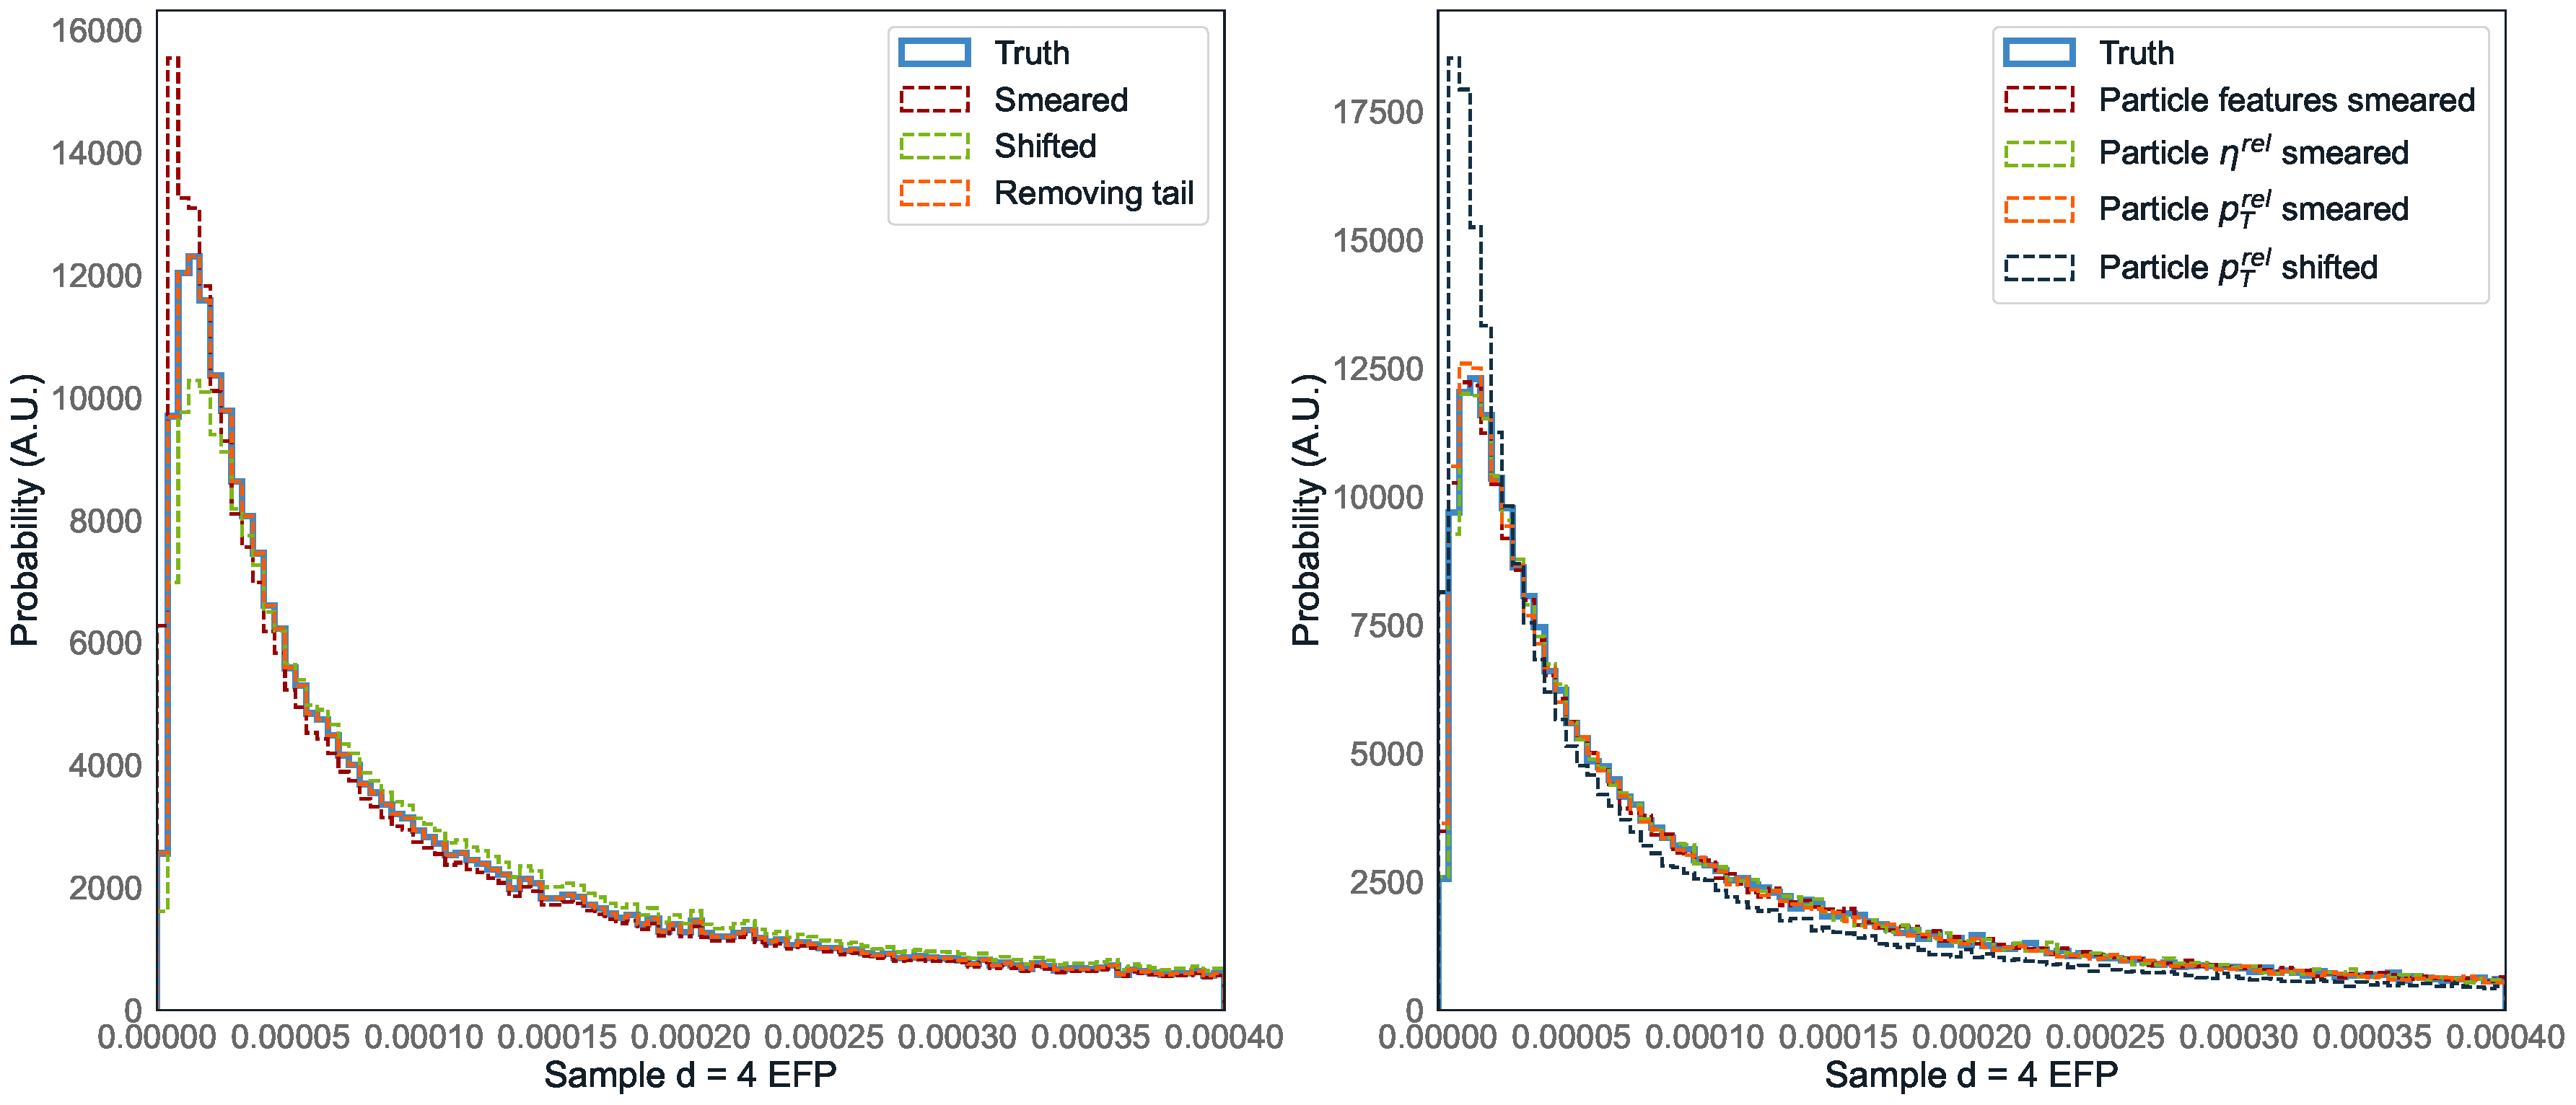
\includegraphics[width=0.94\textwidth]{figures/04-ML4Sim/evaluating/jet_efp25_dists.pdf}
    \caption{The probability, in arbitrary units (A.U.), of the particle \ptrel, a sample $d=3$ EFP, and a sample $d=4$ EFP for truth and distorted gluon jet distributions. 
    On the left are distribution-level distortions, and on the right particle-level.}
    \label{fig:04_evaluating_jet_dists_app}
\end{figure*}